\chapter{Discovering Sparse and Alternative Subgroup Descriptions}
\label{sec:csd}

\section{Overview}
\label{sec:csd:overview}

\paragraph{Scope}

In this chapter, we move to the field of subgroup discovery (cf.~Definition~\ref{def:csd:subgroup-discovery}).
Building on our work regarding constrained feature selection (cf.~Chapter~\ref{sec:syn}), we investigate constraints on features in subgroup descriptions:
We limit the number of selected features and search for alternative solutions, adapting the approach from Chapter~\ref{sec:afs}.
Both these constraint types make subgroup discovery more user-centric.

\paragraph{Contributions}

Our contribution in this chapter is fivefold:

(1) We formalize subgroup discovery as a Satisfiability Modulo Theories (SMT) optimization problem.
This novel white-box formulation admits a solver-based search for subgroups and allows integrating constraints in a declarative manner.

(2) We formalize two constraint types for this optimization problem: feature-cardinality constraints and alternative subgroup descriptions.
\emph{Feature-cardinality constraints} limit the number of selected features, i.e., features used in subgroup descriptions.
Thus, the subgroup descriptions become \emph{sparse}, which increases their interpretability at the potential expense of subgroup quality.
\emph{Alternative subgroup descriptions} should use different features than a given subgroup description but cover a similar set of data objects.
We allow users to control alternatives with two parameters, i.e., the number of alternatives and a dissimilarity threshold.
We integrate both constraint types into our white-box problem formulation.

(3) We describe how to integrate these two constraint types into three existing heuristic search methods and two novel baselines for subgroup discovery.
The latter are faster and simpler than the former, so they may serve as additional reference points for future experimental studies on subgroup discovery.

(4) We analyze the time complexity of the subgroup-discovery problem with each of these two constraint types and prove several $\mathcal{NP}$-completeness results.

(5) We conduct comprehensive experiments with 27 binary-classification datasets from the Penn Machine Learning Benchmarks (PMLB)~\cite{olson2017pmlb, romano2021pmlb}.
We compare solver-based and heuristic subgroup-discovery methods in different experimental scenarios:
without constraints, with a feature-cardinality constraint, and for searching alternative subgroup descriptions.
In particular, we evaluate the runtime of subgroup discovery and the quality of the discovered subgroups.
We also analyze how the subgroup quality in solver-based search depends on the timeout of the solver.
Section~\ref{sec:csd:evaluation:summary} summarizes key results.

\paragraph{Materials}

We publish all our code and experimental data online (cf.~Section~\ref{sec:introduction:materials}).

\paragraph{Prior works}

The content of this chapter bases on the following prior work:
%
\begin{itemize}
	\item \fullcite{bach2024using}
\end{itemize}

\paragraph{Chapter outline}

The remainder of this chapter is structured as follows:
Section~\ref{sec:csd:baselines} introduces two baselines for subgroup discovery.
Section~\ref{sec:csd:approach} describes and analyzes constrained subgroup discovery.
Section~\ref{sec:csd:experimental-design} outlines our experimental design.
Section~\ref{sec:csd:evaluation} presents the corresponding experimental results.

\section{Baselines}
\label{sec:csd:baselines}

In this section, we propose and analyze two baselines for subgroup discovery, \emph{MORS} (cf.~Section~\ref{sec:csd:baselines:mors}) and \emph{Random Search} (cf.~Section~\ref{sec:csd:baselines:random-search}).
They are conceptually simpler than existing heuristic search methods (cf.~Section~\ref{sec:fundamentals:subgroup-discovery:methods}) and serve as further reference points in our experiments.
While they technically also are heuristics, we use the term \emph{baselines} to refer to these two methods specifically.

\begin{algorithm}[t]
	\DontPrintSemicolon
	\KwIn{Dataset~$X \in \mathbb{R}^{m \times n}$, \newline
		Prediction target~$y \in \{0, 1\}^m$
	}
	\KwOut{Subgroup bounds~$\mathit{lb}, \mathit{ub} \in \{\mathbb{R} \cup \{-\infty, +\infty\}\}^n$}
	\BlankLine
	\For{$j \leftarrow 1$ \KwTo $n$}{
		$\mathit{lb}_j \leftarrow \min\limits_{\substack{i \in \{1, \dots, m\} \\ y_i = 1}} X_{ij}$\; \label{al:csd:mors:line:bounds-start}
		$\mathit{ub}_j \leftarrow \max\limits_{\substack{i \in \{1, \dots, m\} \\ y_i = 1}} X_{ij}$\; \label{al:csd:mors:line:bounds-end}
		\lIf{$\mathit{lb}_j = \min_{i \in \{1, \dots, m\}} X_{ij}$}{$\mathit{lb}_j \leftarrow -\infty$} \label{al:csd:mors:line:bounds-infty-start}
		\lIf{$\mathit{ub}_j = \max_{i \in \{1, \dots, m\}} X_{ij}$}{$\mathit{ub}_j \leftarrow + \infty$} \label{al:csd:mors:line:bounds-infty-end}
	}
	\For{$j \notin \text{get\_permissible\_feature\_idxs(\dots)}$}{ \label{al:csd:mors:line:reset-start} \label{al:csd:mors:line:permissible-features}
		$(\mathit{lb}_j,~ \mathit{ub}_j) \leftarrow (-\infty, +\infty)$\; \label{al:csd:mors:line:reset-end}
	}
	\Return{$\mathit{lb}, \mathit{ub}$}
	\caption{\emph{MORS} for subgroup discovery.}
	\label{al:csd:mors}
\end{algorithm}

\subsection{MORS}
\label{sec:csd:baselines:mors}

This baseline builds on the following definition:
%
\begin{definition}[Minimal Optimal-Recall Subgroup (MORS)]
	Given a dataset $X \in \mathbb{R}^{m \times n}$ with prediction target~$y \in \{0, 1\}^m$,
	the \emph{Minimal Optimal-Recall Subgroup (MORS)} is the subgroup (cf.~Definition~\ref{def:csd:subgroup}) whose lower and upper bounds of each feature correspond to the minimum and maximum value of that feature over all positive data objects (i.e., with $y_i = 1$) from the dataset~$X$.
	\label{def:csd:mors}
\end{definition}
%
The definition ensures that all positive data objects are contained in the subgroup.
Thus, the evaluation metric \emph{recall}, i.e., the fraction of positive data objects becoming subgroup members, reaches its \emph{optimal} value of~1.
At the same time, raising the lower bounds or lowering the upper bounds would exclude positive data objects from the subgroup.
In this sense, the set of subgroup members is \emph{minimal}.
The corresponding subgroup description is unique and solves the following variant of the subgroup-discovery problem:
%
\begin{definition}[Minimal-optimal-recall-subgroup discovery]
	Given a dataset $X \in \mathbb{R}^{m \times n}$ with prediction target~$y \in \{0, 1\}^m$,
	\emph{minimal-optimal-recall-subgroup discovery} is the problem of finding a subgroup (cf.~Definition~\ref{def:csd:subgroup}) that contains as few negative data objects (i.e., with $y_i = 0$) as possible but all positive data objects (i.e., with $y_i = 1$) from the dataset~$X$.
	\label{def:csd:minimal-optimal-recall-subgroup-discovery}
\end{definition}
%
I.e., the problem minimizes the number of false positives subject to producing no false negatives.
Equivalently, it maximizes the number of true negatives, i.e., negative data objects excluded from the subgroup, subject to producing no false negatives.

Algorithm~\ref{al:csd:mors} outlines the procedure to determine the \emph{MORS} bounds.
Slightly deviating from Definition~\ref{def:csd:mors}, but consistent to~Algorithm~\ref{al:csd:prim}, \emph{MORS} replaces all non-excluding bounds with infinity (Lines~\ref{al:csd:mors:line:bounds-infty-start}--\ref{al:csd:mors:line:bounds-infty-end}).
Further, if only certain features are permissible to be bounded, as we discuss later, we reset the bounds of the remaining features (Lines~\ref{al:csd:mors:line:reset-start}--\ref{al:csd:mors:line:reset-end}).

Since \emph{MORS} only needs to iterate over all data objects and features once to determine the minima and maxima, the time complexity of this algorithm is~$O(m \cdot n)$.
This places minimal-optimal-recall-subgroup discovery in the complexity class~$\mathcal{P}$:
%
\begin{proposition}[Complexity of minimal-optimal-recall-subgroup discovery]
	The problem of minimal-optimal-recall-subgroup discovery (cf.~Definition~\ref{def:csd:minimal-optimal-recall-subgroup-discovery}) can be solved in~$O(m \cdot n)$.
	\label{prop:csd:complexity-unconstrained-minimal-optimal-recall-subgroup-discovery}
\end{proposition}

Interestingly, a kind of inverted problem definition, the \textsc{Maximum Box} problem, is $\mathcal{NP}$-hard~\cite{eckstein2002maximum}.
The latter problem maximizes the number of true positives, i.e., positive data objects in the subgroup, subject to no false positives, i.e., optimal precision.

For complexity proofs later in this dissertation, we define another variant of the subgroup-discovery problem based on another particular type of subgroups~\cite{meeng2014rocsearch}:
%
\begin{definition}[Perfect subgroup]
	Given a dataset~$X \in \mathbb{R}^{m \times n}$ with prediction target~$y \in \{0, 1\}^m$,
	a \emph{perfect subgroup} is a subgroup (cf.~Definition~\ref{def:csd:subgroup}) that contains all positive data objects (i.e., with $y_i = 1$) but no negative data objects (i.e., with $y_i = 0$) from the dataset~$X$.
	\label{def:csd:perfect-subgroup}
\end{definition}
%
Perfect subgroups reach the theoretical maximum WRAcc (cf.~Equation~\ref{eq:csd:wracc-max}) but do not exist in all datasets.
Next, we define a corresponding search problem:
%
\begin{definition}[Perfect-subgroup discovery]
	Given a dataset~$X \in \mathbb{R}^{m \times n}$ with prediction target~$y \in \{0, 1\}^m$,
	\emph{perfect-subgroup discovery} is the problem of finding a perfect subgroup (cf.~Definition~\ref{def:csd:perfect-subgroup}) if it exists or determining that it does not exist.
	\label{def:csd:perfect-subgroup-discovery}
\end{definition}
%
Since \emph{MORS} helps solving this problem in~$O(m \cdot n)$, we obtain the following result:
%
\begin{proposition}[Complexity of perfect-subgroup discovery]
	The problem of perfect-subgroup discovery (cf.~Definition~\ref{def:csd:perfect-subgroup-discovery}) can be solved in~$O(m \cdot n)$.
	\label{prop:csd:complexity-unconstrained-perfect-subgroup}
\end{proposition}
%
In particular, after \emph{MORS} (cf.~Algorithm~\ref{al:csd:mors}) has found a subgroup, one only needs to check whether it contains any negative data objects.
If it does not, it is perfect, otherwise no perfect subgroup exists.
In particular, the \emph{MORS} bounds cannot be tightened to exclude negative data objects without also excluding positives, thereby violating perfection.

\begin{algorithm}[t]
	\DontPrintSemicolon
	\KwIn{Dataset~$X \in \mathbb{R}^{m \times n}$, \newline
		Prediction target~$y \in \{0, 1\}^m$, \newline
		Subgroup-quality function~$Q(\mathit{lb}, \mathit{ub}, X, y)$, \newline
		Number of iterations~$\mathit{n\_iters} \in \mathbb{N}$
	}
	\KwOut{Subgroup bounds~$\mathit{lb}, \mathit{ub} \in \{\mathbb{R} \cup \{-\infty, +\infty\}\}^n$}
	\BlankLine
	$Q^{\text{opt}} \leftarrow - \infty$\;
	\For{$\mathit{iters} \leftarrow 1$ \KwTo $\mathit{n\_iters}$}{
		\For{$j \leftarrow 1$ \KwTo $n$}{ \label{al:csd:random-search:line:sampling-start}
			$(\mathit{lb}_j,~ \mathit{ub}_j) \leftarrow (-\infty, +\infty)$\;
		}
		\For{$j \in$ get\_permissible\_feature\_idxs(\dots)}{ \label{al:csd:random-search:line:permissible-features}
			$(\mathit{lb}_j,~\mathit{ub}_j) \leftarrow$ sample\_uniformly(unique($X_{\cdot j}$)) \label{al:csd:random-search:line:sampling-end}
		}
		\If{$Q(\mathit{lb}, \mathit{ub}, X, y) > Q^{\text{opt}}$}{ \label{al:csd:random-search:line:optimum-update-start}
			$Q^{\text{opt}} \leftarrow Q(\mathit{lb}, \mathit{ub}, X, y)$\;
			$(\mathit{lb}^{\text{opt}},~ \mathit{ub}^{\text{opt}}) \leftarrow (\mathit{lb},~ \mathit{ub})$\; \label{al:csd:random-search:line:optimum-update-end}
		}
	}
	\For{$j \leftarrow 1$ \KwTo $n$}{ \label{al:csd:random-search:line:bounds-infty-start}
		\lIf{$\mathit{lb}_j^{\text{opt}} = \min_{i \in \{1, \dots, m\}} X_{ij}$}{$\mathit{lb}_j^{\text{opt}} \leftarrow -\infty$} 
		\lIf{$\mathit{ub}_j^{\text{opt}} = \max_{i \in \{1, \dots, m\}} X_{ij}$}{$\mathit{ub}_j^{\text{opt}} \leftarrow +\infty$} \label{al:csd:random-search:line:bounds-infty-end}
	}
	\Return{$\mathit{lb}^{\text{opt}},~ \mathit{ub}^{\text{opt}}$}
	\caption{\emph{Random Search} for subgroup discovery.}
	\label{al:csd:random-search}
\end{algorithm}

\subsection{Random Search}
\label{sec:csd:baselines:random-search}

Algorithm~\ref{al:csd:random-search} outlines a randomized search procedure that constitutes our second baseline.
\emph{Random Search} repeatedly generates and evaluates subgroups for a user-defined number of iterations~$\mathit{n\_iters} \in \mathbb{N}$.
Each generation step samples a lower bound and an upper bound uniformly random from the unique values for each permissible feature, leaving the remaining features unrestricted (Lines~\ref{al:csd:random-search:line:sampling-start}--\ref{al:csd:random-search:line:sampling-end}).
The algorithm tracks the best generated subgroup so far over the iterations (Lines~\ref{al:csd:random-search:line:optimum-update-start}--\ref{al:csd:random-search:line:optimum-update-end}) and finally returns it.
As for Algorithm~\ref{al:csd:prim}, \emph{Random Search} replaces all non-excluding bounds with infinity (Lines~\ref{al:csd:random-search:line:bounds-infty-start}--\ref{al:csd:random-search:line:bounds-infty-end}).

\section{Constrained Subgroup Discovery}
\label{sec:csd:approach}

In this section, we discuss subgroup discovery with constraints.
First, we frame subgroup discovery as an SMT optimization problem (cf.~Section~\ref{sec:csd:approach:smt}).
Second, we formalize and analyze feature-cardinality constraints (cf.~Section~\ref{sec:csd:approach:cardinality}).
Third, we formalize and analyze alternative subgroup descriptions (cf.~Section~\ref{sec:csd:approach:alternatives}).

\subsection{SMT Encoding of Subgroup Discovery}
\label{sec:csd:approach:smt}

To find optimal subgroups exactly, one can encode subgroup discovery as a white-box optimization problem and employ a solver.
As for constrained feature selection, this approach allows directly integrating and combining a variety of constraint types in a declarative manner.
Similar to Section~\ref{sec:syn:approach}, we propose an SMT encoding with linear real arithmetic (LRA)~\cite{barrett2018satisfiability}.
This formulation is straightforward given the problem definition (cf.~Definition~\ref{def:csd:subgroup-discovery}).
Appendix~\ref{sec:appendix:csd:milp-encoding} describes an encoding as a mixed integer linear program (MILP), which performed worse in preliminary experiments.
Beyond the scope of this dissertation, \cite{bach2024using}~outlines a \textsc{MaxSAT} encoding and how to handle categorical features.

The optimization problem consists of an objective function and constraints.

\paragraph{Objective function}

We use WRAcc as the objective, which should be maximized.
In the formula for WRAcc (cf.~Equation~\ref{eq:csd:wracc}), $m$ and $m^+$ are constants, while $m_b$ and $m_b^+$ depend on the decision variables.
The previously provided formula contains $m_b$ in the numerator and denominator, but one can reformulate it by multiplying its two factors:
%
\begin{equation}
	\text{WRAcc} = \frac{m_b^+}{m} - \frac{m_b \cdot m^+}{m^2} = \frac{m_b^+ \cdot m - m_b \cdot m^+}{m^2}
	\label{eq:csd:smt-wracc}
\end{equation}
%
In this new expression, the denominators and the factor~$m^+$ in the numerator are constant.
Thus, the whole expression is linear in~$m_b^+$ and~$m_b$.
We define these two quantities as linear expressions from binary decision variables~$b \in \{0, 1\}^m$ that denote subgroup membership.
I.e., $b_i$~expresses whether the $i$-th data object is in the subgroup.
%
\begin{equation}
	\begin{aligned}
		m_b &:= \sum_{i=1}^{m} b_i \\
		m_b^+ &:= \sum_{\substack{i \in \{1, \dots, m\} \\ y_i = 1 }} b_i \\
	\end{aligned}
	\label{eq:csd:smt-constraint-m-as-sum}
\end{equation}
%
Since the values of the target variable~$y$ are fixed, the expression for~$m_b^+$ only sums over the positive data objects.
Further, one may define $m_b^+$ and~$m_b$ as separate integer variables or directly insert their expressions into Equation~\ref{eq:csd:smt-wracc}.
We chose the latter in our implementation and therefore wrote `$:=$' in Equation~\ref{eq:csd:smt-constraint-m-as-sum} instead of using a propositional operator like `$\leftrightarrow$'.
Finally, the formula for nWRAcc (cf.~Equation~\ref{eq:csd:wracc-normalized}) is linear as well, having the same enumerator as Equation~\ref{eq:csd:smt-wracc} and a different constant in the denominator.

\paragraph{Constraints}

The subgroup membership~$b_i$ of a data object depends on the bounds of the subgroup (cf.~Definition~\ref{def:csd:subgroup}).
Thus, we define real-valued decision variables $\mathit{lb}, \mathit{ub} \in \{\mathbb{R} \cup \{-\infty, +\infty\}\}^n$ for the latter.
In particular, each feature has a lower bound and an upper bound.
The upper bounds naturally need to be at least as high as the lower bounds:
%
\begin{equation}
	\forall j \in \{1, \dots, n\}:~ \mathit{lb}_j\leq \mathit{ub}_j
	\label{eq:csd:smt-constraint-bounds-monotonic}
\end{equation}
%
A data object is a member of the subgroup if all its feature values are within the bounds:
%
\begin{equation}
	\forall i \in \{1, \dots, m\}:~ b_i\leftrightarrow \bigwedge_{j \in \{1, \dots, n\}} \left( \left( X_{ij} \geq \mathit{lb}_j \right) \land \left( X_{ij} \leq \mathit{ub}_j \right) \right)
	\label{eq:csd:smt-constraint-subgroup-membership}
\end{equation}
%
Instead of defining separate decision variables~$b_i$ and binding them to the bounds with an equivalence constraint, one could also insert the corresponding Boolean expression into the right-hand-side of Equation~\ref{eq:csd:smt-constraint-m-as-sum} directly.
In particular, $\mathit{lb}_j$ and $\mathit{ub}_j$ are the only decision variables strictly necessary for the optimization problem.
However, some constraint types on subgroups may use~$b_i$ as well, so it is helpful to have it defined explicitly.

\paragraph{Complete optimization problem}

Combining all prior definitions of decision variables, constraints, and the objective, we obtain the following SMT optimization problem:

\begin{equation}
	\begin{aligned}
		\max &\quad & Q_{\text{WRAcc}} &= \frac{m_b^+}{m} - \frac{m_b \cdot m^+}{m^2} \\
		\text{s.t.:} &\quad & m_b &:= \sum_{i=1}^{m} b_i \\
		&\quad & m_b^+ &:= \sum_{\substack{i \in \{1, \dots, m\} \\ y_i = 1 }} b_i \\
		&\quad \forall i \in \{1, \dots, m\} & b_i &\leftrightarrow \bigwedge_{j \in \{1, \dots, n\}} \left( \left( X_{ij} \geq \mathit{lb}_j \right) \land \left( X_{ij} \leq \mathit{ub}_j \right) \right) \\
		&\quad \forall j \in \{1, \dots, n\} & \mathit{lb}_j &\leq \mathit{ub}_j \\
		&\quad & b &\in \{0, 1\}^m \\
		&\quad & \mathit{lb}, \mathit{ub} &\in \{\mathbb{R} \cup \{-\infty, +\infty\}\}^n
	\end{aligned}
	\label{eq:csd:smt-problem-unconstrained-complete}
\end{equation}

We refer to this optimization problem as \emph{unconstrained subgroup discovery} in the following since it only contains constraints to define subgroup discovery per se but not the additional constraints on feature sets that we will impose later.

\paragraph{Post-processing}

In our implementation, we add a small post-processing step.
In particular, we do not use the solver-determined values of the variables $\mathit{lb}_j$ and $\mathit{ub}_j$ but the minimum and maximum feature values of all data objects in the subgroup (i.e., with $b_i=1$).
Thus, we ensure that the bounds correspond to actual feature values, consistent with the bounds returned by heuristic search methods and baselines.
Further, this choice avoids potential numerical issues caused by extracting floating-point values from the solver.
If the subgroup does not contain any data objects, we use invalid bounds (i.e., $\mathit{ub}_j = -\infty < \infty = \mathit{lb}_j$) to ensure that the subgroup remains empty even for arbitrary new data objects.

\subsection{Feature-Cardinality Constraints}
\label{sec:csd:approach:cardinality}

In this section, we discuss feature-cardinality constraints for subgroup discovery.
First, we motivate and formalize them (cf.~Section~\ref{sec:csd:approach:cardinality:concept}).
Next, we describe how to integrate them into our SMT encoding of subgroup discovery (cf.~Section~\ref{sec:csd:approach:cardinality:smt}), heuristic search methods (cf.~Section~\ref{sec:csd:approach:cardinality:heuristics}), and baselines (cf.~Section~\ref{sec:csd:approach:cardinality:baselines}).
Finally, we analyze the time complexity of subgroup discovery with this constraint type (cf.~Section~\ref{sec:csd:approach:cardinality:complexity}).

\subsubsection{Concept}
\label{sec:csd:approach:cardinality:concept}

Feature-cardinality constraints limit the number of features used in the subgroup description, rendering the latter less complex and easier to interpret~\cite{meeng2021real}.
To formalize this constraint type, we define feature selection in subgroup discovery as follows:
%
\begin{definition}[Feature selection in subgroups]
	Given a dataset~$X \in \mathbb{R}^{m \times n}$ and a subgroup (cf.~Definition~\ref{def:csd:subgroup}) with bounds~$\mathit{lb}, \mathit{ub} \in \{\mathbb{R} \cup \{-\infty, +\infty\}\}^n$,
	Feature~$j$ is \emph{selected} if the bounds exclude at least one data object of~$X$ from the subgroup, i.e., $\exists i \in \{1, \dots, m\}:~ \left( X_{ij} < \mathit{lb}_j \right) \lor \left( X_{ij} > \mathit{ub}_j \right)$.
	\label{def:csd:feature-selection}
\end{definition}
%
The bounds of unselected features can be considered infinite, effectively removing these features from the subgroup description.
The \emph{feature cardinality} of the subgroup is the number of selected features.
Related work (cf.~Section~\ref{sec:related-work:constraints:subgroup-discovery}) also uses the terms \emph{depth} \cite{meeng2021real} or \emph{length} \cite{atzmueller2015subgroup, helal2016subgroup}, though partly referring to the number of conditions in the subgroup description rather than selected features.
I.e., if there is a lower and an upper bound for a feature, some related work counts this feature twice instead of once.

Feature-cardinality constraints employ a user-defined limit on feature cardinality:
%
\begin{definition}[Feature-cardinality constraint]
	Given a cardinality threshold $k \in \mathbb{N}$,
	a \emph{feature-cardinality constraint} for a subgroup (cf.~Definition~\ref{def:csd:subgroup}) requires the subgroup to have at most $k$~features selected (cf.~Definition~\ref{def:csd:feature-selection}).
	\label{def:csd:feature-cardinality-constraint}
\end{definition}
%
In some scenarios, selecting less than exactly $k$ features may improve subgroup quality.
Thus, we use an inequality rather than the equality (cf.~Equation~\ref{eq:syn:cardinality}) we employed in our work on alternative feature selection (cf.~Chapter~\ref{sec:afs}).

\subsubsection{SMT Encoding}
\label{sec:csd:approach:cardinality:smt}

We first need to encode whether a feature is selected or not.
Thus, we introduce binary decision variables $s, s^{\text{lb}}, s^{\text{ub}} \in \{0, 1\}^n$.
A feature is selected if its bounds exclude at least one data object from the subgroup (cf.~Definition~\ref{def:csd:feature-selection}), i.e., the lower bound is higher than the minimum feature value or the upper bound is lower than the maximum feature value:
%
\begin{equation}
	\begin{aligned}
		\forall j: & & s^{\text{lb}}_j &\leftrightarrow \left( \mathit{lb}_j > \min_{i \in \{1, \dots, m\}} X_{ij} \right) \\
		\forall j: & &s^{\text{ub}}_j &\leftrightarrow \left( \mathit{ub}_j < \max_{i \in \{1, \dots, m\}} X_{ij} \right) \\
		\forall j: & & s_j &\leftrightarrow \left( s^{\text{lb}}_j \lor s^{\text{ub}}_j \right) \\
		\text{with index:} & & j &\in \{1, \dots, n\}
	\end{aligned}
	\label{eq:csd:smt-constraint-feature-selection}
\end{equation}
%
In this equation, minimum and maximum feature values are constants that can be determined before formulating the optimization problem.
Given the definition of~$s_j$, setting an upper bound on the number of selected features (cf.~Definition~\ref{def:csd:feature-cardinality-constraint}) is straightforward:
%
\begin{equation}
	\sum_{j=1}^n s_j \leq k
	\label{eq:csd:smt-constraint-feature-cardinalty}
\end{equation}
%
Instead of defining the decision variables $s_j$, $s^{\text{lb}}_j$, and $s^{\text{ub}}_j$, one could also insert the corresponding expressions into Equation~\ref{eq:csd:smt-constraint-feature-cardinalty} directly.
However, we will also use~$s_j$ for alternative subgroup descriptions (cf.~Section~\ref{sec:csd:approach:alternatives:smt}), so we define corresponding variables.

The overall SMT encoding of subgroup discovery with a feature-cardinality constraint is the SMT encoding of unconstrained subgroup discovery (cf.~Equation~\ref{eq:csd:smt-problem-unconstrained-complete}) supplemented by the variables and constraints from Equations~\ref{eq:csd:smt-constraint-feature-selection} and~\ref{eq:csd:smt-constraint-feature-cardinalty}.
Our implementation also contains a post-processing step that sets non-excluding lower bounds (i.e., with $s^{\text{lb}}_j = 0$) to $-\infty$ and non-excluding upper bounds (i.e., with $s^{\text{ub}}_j = 0$) to $+\infty$.
This step is consistent with the heuristic search methods and baselines (e.g., cf.~Lines~\ref{al:csd:prim:line:bounds-infty-start}--\ref{al:csd:prim:line:bounds-infty-end} in Algorithm~\ref{al:csd:prim}).

\subsubsection{Integration into Heuristic Search Methods}
\label{sec:csd:approach:cardinality:heuristics}

The feature-cardinality constraint (cf.~Definition~\ref{def:csd:feature-cardinality-constraint}) is \emph{antimonotonic}~\cite{ng1998exploratory} in the feature selection:
If a selected feature set satisfies the constraint, all its subsets also satisfy it.
Vice versa, if a feature set violates the constraint, all its supersets also violate it.
This property allows to easily integrate the constraint into the three heuristic search methods from Section~\ref{sec:fundamentals:subgroup-discovery:methods}, i.e., \emph{PRIM} (cf.~Algorithm~\ref{al:csd:prim}), \emph{Beam Search} (cf.~Algorithms~\ref{al:csd:generic-beam-search} and~\ref{al:csd:beam-search-subgroup-update}), and \emph{Best Interval} (cf.~Algorithms~\ref{al:csd:generic-beam-search} and~\ref{al:csd:best-interval-subgroup-update}), which all iteratively enlarge the set of selected features.
In particular, these search methods start with unrestricted subgroup bounds, i.e., an empty feature set, which satisfies the constraint for any~$k \geq 0$.
Each iteration may either add bounds on one further feature or refine the bounds on an already selected feature.
Thus, one can prevent generation of invalid solution candidates by defining the function \emph{get\_permissible\_feature\_idxs(\dots)} (cf.~Line~\ref{al:csd:prim:line:permissible-features} in Algorithm~\ref{al:csd:prim} and Line~\ref{al:csd:generic-beam-search:line:permissible-features} in Algorithm~\ref{al:csd:generic-beam-search}) as follows:
If already $k$~features are selected, only these features are permissible.
If less than $k$~features are selected, all features are permissible, as in the unconstrained search.

\subsubsection{Integration into Baselines}
\label{sec:csd:approach:cardinality:baselines}

\paragraph{MORS}

\emph{MORS} calls the function \emph{get\_permissible\_feature\_idxs(\dots)} in Line~\ref{al:csd:mors:line:permissible-features} of Algorithm~\ref{al:csd:mors}.
To instantiate this function, we employ a univariate, quality-based heuristic for feature selection:
For each feature, we evaluate what would happen if only this feature was restricted according to \emph{MORS} (cf.~Definition~\ref{def:csd:mors}).
In particular, we determine the number of false positives, i.e., negative data objects in the subgroup, defined by each feature's \emph{MORS} bounds (Lines~\ref{al:csd:mors:line:bounds-start}--\ref{al:csd:mors:line:bounds-end}).
We select the $k$~features with the lowest number of false positives.

This heuristic is equivalent to selecting the features with the highest WRAcc for univariate \emph{MORS} bounds:
Due to \emph{MORS}, not only~$m$ and~$m^+$ are constant but also the number of positive subgroup members~$m_b^+$, which equals~$m^+$.
Thus, one can rephrase Equation~\ref{eq:csd:wracc}:
%
\begin{equation}
	\text{WRAcc}_{\text{MORS}} = \frac{m_b^+}{m} - \frac{m_b \cdot m^+}{m^2} = \frac{m^+}{m} - \frac{m_b \cdot m^+}{m^2} = \frac{m^+}{m} \cdot \left( 1 - \frac{m_b}{m} \right)
	\label{eq:csd:wracc-mors}
\end{equation}
%
Thus, maximizing WRAcc corresponds to minimizing~$m_b / m$, i.e., the relative frequency of the data objects in the subgroup.
Since the number of positive data objects in the subgroup is fixed in \emph{MORS}, this objective amounts to including as few negative data objects as possible in the subgroup, i.e., minimizing the number of false positives like our heuristic.

\paragraph{Random Search}

\emph{Random Search} calls \emph{get\_permissible\_feature\_idxs(\dots)} in Line~\ref{al:csd:random-search:line:permissible-features} of Algorithm~\ref{al:csd:random-search}).
To observe a cardinality threshold~$k$, we simply sample~$k$ out of $n$ features uniformly random without replacement.
The bounds for these features will be restricted in the next step of the algorithm, while all remaining features remain unrestricted.

\subsubsection{Time Complexity}
\label{sec:csd:approach:cardinality:complexity}

We analyze three aspects of time complexity:
the size of the search space for exhaustive search, parameterized complexity, and $\mathcal{NP}$-hardness.

\paragraph{Exhaustive search}

Before addressing feature-cardinality constraints, we analyze the unconstrained case.
In general, the search space of subgroup discovery depends on the number of candidates for lower and upper bounds.
With $m$~data objects, each real-valued feature may have up to $m$~unique values.
It suffices to treat these unique values as bound candidates since any bounds between feature values or outside the feature's range do not change the subgroup membership during optimization.
Thus, there are $O(m^2)$ relevant lower-upper-bound combinations per feature.
Since we need to combine bounds over all $n$~features, the size of the search space is $O(m^{2n})$:
%
\begin{proposition}[Complexity of exhaustive search for subgroup discovery]
	An exhaustive search for subgroup discovery (cf.~Definition~\ref{def:csd:subgroup-discovery}) needs to evaluate $O(m^{2n})$ subgroups.
	\label{prop:csd:complexity-unconstrained-exhaustive}
\end{proposition}
%
For each of these candidate subgroups, the cost of evaluating a quality function like WRAcc (cf.~Equation~\ref{eq:csd:wracc}) typically is $O(m \cdot n)$, i.e., requires a constant number of passes over the dataset and therefore has linear complexity in the dataset size.
Further, the number of potential subgroups only is an upper bound:
Efficient exhaustive search methods employ quality-based pruning to not evaluate all solution candidates explicitly~\cite{atzmueller2015subgroup}.

Next, we adapt the result from Proposition~\ref{prop:csd:complexity-unconstrained-exhaustive} to feature-cardinality constraints.
There are $\binom{n}{k} \leq n^k$ feature sets of size~$k$ with $O(m^{2k})$ bound candidates each:
%
\begin{proposition}[Complexity of exhaustive search for subgroup discovery with feature-cardinality constraint]
	An exhaustive search for subgroup discovery (cf.~Definition~\ref{def:csd:subgroup-discovery}) with a feature-cardinality constraint (cf.~Definition~\ref{def:csd:feature-cardinality-constraint}) needs to evaluate $O(n^k \cdot m^{2k})$ subgroups.
	\label{prop:csd:complexity-cardinality-exhaustive}
\end{proposition}
%
For the special case $k=1$, the size of the search space becomes $O(n \cdot m^2)$, which is implicitly leveraged by heuristic search methods that only consider updating the bounds of each feature separately instead of jointly (cf.~Section~\ref{sec:fundamentals:subgroup-discovery:methods}).

\paragraph{Parameterized complexity}

If we consider the number of features~$n$ to be a small constant, the search-space size of unconstrained subgroup discovery (cf.~Proposition~\ref{prop:csd:complexity-unconstrained-exhaustive}) is polynomial in~$m$ and thereby also polynomial in the dataset size $m \cdot n$.
Thus, the problem of subgroup discovery belongs to the parameterized complexity class $\mathcal{XP}$~\cite{downey1997parameterized}:
%
\begin{proposition}[Parameterized complexity of subgroup discovery]
	The problem of subgroup discovery (cf.~Definition~\ref{def:csd:subgroup-discovery}) resides in the parameterized complexity class~$\mathcal{XP}$ for the parameter~$n$.
	\label{prop:csd:complexity-unconstrained-xp}
\end{proposition}
%
In contrast, the complexity remains exponential in~$n$ if $m$~is fixed.
I.e., the number of features has an exponential impact on the size of the search space, while the number of data objects has a polynomial impact.
With a feature-cardinality constraint, the problem retains its $\mathcal{XP}$ membership.
Considering the size of the search space from Proposition~\ref{prop:csd:complexity-cardinality-exhaustive}, the parameter is~$k$ instead of~$n$ now:
%
\begin{proposition}[Parameterized complexity of subgroup discovery with feature-cardinality constraint]
	The problem of subgroup discovery (cf.~Definition~\ref{def:csd:subgroup-discovery}) with a feature-cardinality constraint (cf.~Definition~\ref{def:csd:feature-cardinality-constraint}) resides in the parameterized complexity class~$\mathcal{XP}$ for the parameter~$k$.
	\label{prop:csd:complexity-cardinality-xp}
\end{proposition}

\paragraph{NP-Hardness}

\cite{boley2009non} showed $\mathcal{NP}$-hardness for finding a subgroup description with minimum feature cardinality that replicates the membership of a given subgroup.
We transfer this result to optimizing subgroup quality under a feature-cardinality constraint.
First, we tackle the search problem for perfect subgroups (cf.~Appendix~\ref{sec:appendix:csd:proofs:complexity-cardinality-np-perfect-subgroup} for the proof):
%
\begin{proposition}[Complexity of perfect-subgroup discovery with feature-cardinality constraint]
	The problem of perfect-subgroup discovery (cf.~Definition~\ref{def:csd:perfect-subgroup-discovery}) with a feature-cardinality constraint (cf.~Definition~\ref{def:csd:feature-cardinality-constraint}) is $\mathcal{NP}$-complete.
	\label{prop:csd:complexity-cardinality-np-perfect-subgroup}
\end{proposition}
%
This hardness result contrasts with the polynomial runtime of unconstrained perfect-subgroup discovery (cf.~Proposition~\ref{prop:csd:complexity-unconstrained-perfect-subgroup}), which corresponds to a cardinality constraint with $k = n$.
Generalizing Proposition~\ref{prop:csd:complexity-cardinality-np-perfect-subgroup}, the optimization problem of subgroup discovery with a feature-cardinality constraint is $\mathcal{NP}$-complete under a reasonable assumption on the notion of subgroup quality (cf.~Appendix~\ref{sec:appendix:csd:proofs:complexity-cardinality-np} for the proof):
%
\begin{proposition}[Complexity of subgroup discovery with feature-cardinality constraint]
	Assuming a subgroup-quality function~$Q(\mathit{lb}, \mathit{ub}, X, y)$ for which only perfect subgroups (cf.~Definition~\ref{def:csd:perfect-subgroup}) reach its maximal value,
	the problem of subgroup discovery (cf.~Definition~\ref{def:csd:subgroup-discovery}) with a feature-cardinality constraint (cf.~Definition~\ref{def:csd:feature-cardinality-constraint}) is $\mathcal{NP}$-complete.
	\label{prop:csd:complexity-cardinality-np}
\end{proposition}
%
WRAcc as the subgroup-quality function satisfies this assumption since only perfect subgroups yield the theoretical maximum WRAcc (cf.~Equation~\ref{eq:csd:wracc-max}).

\subsection{Alternative Subgroup Descriptions}
\label{sec:csd:approach:alternatives}

In this section, we propose the optimization problem of discovering alternative subgroup descriptions.
First, we motivate and formalize the problem (cf.~Section~\ref{sec:csd:approach:alternatives:concept}).
Next, we describe how to phrase it within our SMT encoding of subgroup discovery (cf.~Section~\ref{sec:csd:approach:alternatives:smt}), heuristic search methods (cf.~Section~\ref{sec:csd:approach:alternatives:heuristics}), and baselines (cf.~Section~\ref{sec:csd:approach:alternatives:baselines}).
Finally, we analyze the time complexity of this problem (cf.~Section~\ref{sec:csd:approach:alternatives:complexity}).

\subsubsection{Concept}
\label{sec:csd:approach:alternatives:concept}

\paragraph{Overview}

For alternative subgroup descriptions, we assume to have an \emph{original subgroup} given, with subgroup membership~$b^{(0)} \in \{0, 1\}^m$ of data objects and with feature selection~$s^{(0)} \in \{0, 1\}^n$.
When searching alternatives, we do not optimize subgroup quality but the similarity to this original subgroup.
We express the similarity in terms of subgroup membership.
If this similarity is very high, then the subgroup quality should also be similar since evaluation metrics for subgroup quality typically base on subgroup membership.

Additionally, we constrain the new subgroup description to be alternative enough.
We express this dissimilarity in terms of the subgroups' feature selection.
The user chooses a dissimilarity threshold~$\tau \in \mathbb{R}_{\geq 0}$ and can thereby control alternatives.
Further, we recommend employing a feature-cardinality constraint (cf.~Definition~\ref{def:csd:feature-cardinality-constraint}) when determining the original subgroup so there are sufficiently many features left for the alternative.
The alternative may be feature-cardinality-constrained as well, to increase its interpretability.

In a nutshell, alternative subgroup descriptions should produce similar subgroup membership as the original subgroup but use different features.

\paragraph{Sequential search}

One can search for multiple alternative subgroup descriptions sequentially, as for alternative feature sets (cf.~Section~\ref{sec:afs:approach:constraints:multiple}).
After determining the original subgroup, each iteration yields one further alternative.
Users may prescribe a number of alternatives~$a \in \mathbb{N}$ a priori or stop the procedure whenever the alternatives are not interesting anymore, e.g., too dissimilar to the original subgroup.
Each alternative should have a similar subgroup membership as the original subgroup but a dissimilar feature selection compared to all \emph{existing subgroups} found in prior iterations:
%
\begin{definition}[Alternative-subgroup-description discovery]
	Given
	\begin{itemize}[noitemsep]
		\item a dataset $X \in \mathbb{R}^{m \times n}$,
		\item $a \in \mathbb{N}$ existing subgroups with subgroup membership~$b^{(l)} \in \{0, 1\}^m$ and feature selection~$s^{(l)} \in \{0, 1\}^n$ for $l \in \{0, \dots, a - 1\}$,
		\item a similarity measure $\text{sim}(\cdot)$ for subgroup-membership vectors,
		\item a dissimilarity measure $\text{dis}(\cdot)$ for feature-selection vectors of subgroups,
		\item and a dissimilarity threshold~$\tau \in \mathbb{R}_{\geq 0}$,
	\end{itemize}
	\emph{alternative-subgroup-description discovery} is the problem of finding a subgroup (cf.~Definition~\ref{def:csd:subgroup}) with membership~$b^{(a)} \in \{0, 1\}^m$ and feature selection~$s^{(a)} \in \{0, 1\}^n$ that maximizes the subgroup-membership similarity $\text{sim}(b^{(a)}, b^{(0)})$ to the original subgroup while being dissimilar to all existing subgroups regarding the feature selection, i.e., $\forall l \in \{0, \dots, a-1\}:~\text{dis}(s^{(a)}, s^{(l)}) \geq \tau$.
	\label{def:csd:alternative-subgroup-description-discovery}
\end{definition}
%
Compared to the conventional subgroup-discovery problem (cf.~Definition~\ref{def:csd:subgroup-discovery}), $b^{(0)}$ replaces the prediction target~$y$, and $\text{sim}(\cdot)$ replaces the subgroup-quality function~$Q(\mathit{lb}, \mathit{ub}, X, y)$.
In the following, we discuss $\text{sim}(\cdot)$ and $\text{dis}(\cdot)$.

\paragraph{Similarity in objective function}

There are various options to quantify the similarity of subgroup membership, i.e., between two binary vectors.
For example, the Hamming distance counts how many vector entries differ~\cite{choi2010survey}.
We turn this distance into a similarity measure by counting identical vector entries.
Further, we normalize the similarity with the vector length, i.e., number of data objects~$m$, to obtain the following \emph{normalized Hamming similarity} for two subgroup-membership vectors~$b', b'' \in \{0, 1\}^m$:
%
\begin{equation}
	\text{sim}_{\text{nHamm}}(b', b'') = \frac{1}{m} \cdot \sum_{i=1}^{m} (b'_i = b''_i)
	\label{eq:csd:hamming-general}
\end{equation}
%
If either $b'$ or $b''$ is constant, this similarity measure is linear in its remaining argument, as discussed later (cf.~Equation~\ref{eq:csd:smt-hamming}).
Further, if one considers one vector to be a prediction and the other to be the ground truth, Equation~\ref{eq:csd:hamming-general} equals prediction accuracy for classification.
Another popular similarity measure for sets or binary vectors is the Jaccard index (cf.~Equation~\ref{eq:afs:jaccard}), which relates the intersection of positive vector entries to their union:
%
\begin{equation}
	\text{sim}_{\text{Jacc}}(b', b'') = \frac{\sum_{i=1}^{m} (b'_i \land b''_i)}{\sum_{i=1}^{m} (b'_i \lor b''_i)}
	\label{eq:csd:jaccard}
\end{equation}
%
However, this similarity measure is not linear in~$b'$ and~$b''$, which prevents its use in certain white-box solvers.
Thus, we use the normalized Hamming similarity.

\paragraph{Dissimilarity in constraints}

For the dissimilarity between feature-selection vectors, we employ the following \emph{deselection dissimilarity} with an adapted dissimilarity threshold:
%
\begin{equation}
	\text{dis}_{\text{des}}(s^{\text{new}}, s^{\text{old}}) = \sum_{j=1}^n (\lnot s^{\text{new}}_j \land s^{\text{old}}_j) \geq \min \left( \tau_{\text{abs}},~k^{\text{old}} \right)
	\label{eq:csd:constraint-dissimilarity}
\end{equation}
%
This dissimilarity counts how many previously selected features are \emph{not} selected in the new subgroup description.
These features may either be replaced by other features, or the total number of selected features may be reduced.
The constraint ensures that at least $\tau_{\text{abs}} \in \mathbb{N}_0$ features are deselected but never more than there were selected before ($k^{\text{old}}$), which would be infeasible.
For maximum dissimilarity, none of the previously selected features may be selected again.
This dissimilarity measure is asymmetric, i.e., $\text{dis}_{\text{des}}(s^{\text{new}}, s^{\text{old}}) \neq \text{dis}_{\text{des}}(s^{\text{old}}, s^{\text{new}})$, which would be an issue in a simultaneous search for alternatives but is acceptable in sequential search, where `old' and `new' are well-defined.

Compared to more common dissimilarity measures like the Jaccard distance or the Dice dissimilarity (cf.~Equation~\ref{eq:afs:dice}), our deselection dissimilarity has two advantages:
First, if $s^{\text{old}}$ is constant, the dissimilarity is a simple sum and therefore linear in $s^{\text{new}}$, even if the number of newly selected features is unknown yet, while Jaccard distance and Dice dissimilarity involve a ratio in the latter case.
This property is useful for solver-based search (cf.~Section~\ref{sec:csd:approach:alternatives:smt}).
Second, Equation~\ref{eq:csd:constraint-dissimilarity} is antimonotonic in the new feature selection, which is useful for heuristic search (cf.~Section~\ref{sec:csd:approach:alternatives:heuristics}).
Using the Jaccard distance or Dice dissimilarity in the constraint violates this property.
In particular, these dissimilarities can increase by selecting features that were not selected before, i.e., an invalid feature set can become valid instead of remaining invalid by selecting further features.

\subsubsection{SMT Encoding}
\label{sec:csd:approach:alternatives:smt}

Slightly reformulating Equation~\ref{eq:csd:hamming-general} yields a linear objective function regarding~$b^{(a)}$:
%
\begin{equation}
	\begin{aligned}
		\text{sim}_{\text{nHamm}}(b^{(a)}, b^{(0)}) &= \frac{1}{m} \cdot \sum_{i=1}^m \left( b_i^{(a)} \leftrightarrow b_i^{(0)} \right) \\
		&= \frac{1}{m} \cdot \Big( \sum\limits_{\substack{i \in \{1, \dots, m\} \\ b_i^{(0)} = 1}} b_i^{(a)} + \sum\limits_{\substack{i \in \{1, \dots, m\} \\ b_i^{(0)} = 0}} \lnot b_i^{(a)} \Big)
	\end{aligned}
	\label{eq:csd:smt-hamming}
\end{equation}
%
In particular, since $b^{(0)}$~is known and therefore constant, we employ the expression from the second line, i.e., without the logical equivalence operator.
Instead, we compute two sums, one for data objects that are members of the original subgroup and one for non-members.
The negated expression $\lnot b_i^{(a)}$ may be expressed as $1 - b_i^{(a)}$.

To formulate the dissimilarity constraints, we leverage that the feature-selection vector~$s^{(l)}$ and the corresponding number of selected features~$k^{(l)}$ are known for all existing subgroups as well.
Thus, we instantiate and adapt Equation~\ref{eq:csd:constraint-dissimilarity} as follows:

\begin{equation}
	\forall l \in \{0, \dots, a-1\}:~ \text{dis}_{\text{des}}(s^{(a)}, s^{(l)}) = \sum_{\substack{j \in \{1, \dots, n\} \\ s^{(l)}_j = 1}} \lnot s^{(a)}_j \geq \min \left( \tau_{\text{abs}},~k^{(l)} \right)
	\label{eq:csd:smt-constraint-dissimilarity}
\end{equation}
%
In particular, we only sum over features that were selected in the existing subgroup and check whether they are deselected now.

The overall SMT encoding of alternative-subgroup-description discovery (cf.~Definition~\ref{def:csd:alternative-subgroup-description-discovery}) combines the similarity objective (cf.~Equation~\ref{eq:csd:smt-hamming}) and dissimilarity constraints (cf.~Equation~\ref{eq:csd:smt-constraint-dissimilarity}) with the previously introduced variables and constraints for bounds (cf.~Equation~\ref{eq:csd:smt-constraint-bounds-monotonic}), subgroup membership (cf.~Equation~\ref{eq:csd:smt-constraint-subgroup-membership}), and feature selection (cf.~Equation~\ref{eq:csd:smt-constraint-feature-selection}).
Optionally, one may add a feature-cardinality constraint (cf.~Equation~\ref{eq:csd:smt-constraint-feature-cardinalty}).

\subsubsection{Integration into Heuristic Search Methods}
\label{sec:csd:approach:alternatives:heuristics}

The situation is similar to integrating feature-cardinality constraints (cf.~Section~\ref{sec:csd:approach:cardinality:heuristics}).
In particular, the constraint for alternatives based on the deselection dissimilarity (cf.~Equation~\ref{eq:csd:constraint-dissimilarity}) is antimonotonic.
I.e., the constraint is satisfied for an empty feature set, and once it is violated for a feature set, it remains violated for any superset.
Thus, the constraint type is suitable for heuristic search methods that iteratively enlarge the set of selected features, like \emph{PRIM} (cf.~Algorithm~\ref{al:csd:prim}), \emph{Beam Search} (cf.~Algorithms~\ref{al:csd:generic-beam-search} and~\ref{al:csd:beam-search-subgroup-update}), and \emph{Best Interval} (cf.~Algorithms~\ref{al:csd:generic-beam-search} and~\ref{al:csd:best-interval-subgroup-update}).
We only need to adapt the function \emph{get\_permissible\_feature\_idxs(\dots)} (cf.~Line~\ref{al:csd:prim:line:permissible-features} in Algorithm~\ref{al:csd:prim} and Line~\ref{al:csd:generic-beam-search:line:permissible-features} in Algorithm~\ref{al:csd:generic-beam-search}) to return the indices of all features that may be selected without violating the dissimilarity constraint (cf.~Equation~\ref{eq:csd:constraint-dissimilarity}).
In particular, once $k^{(l)} - \tau_{\text{abs}}$~features from an existing subgroup with $k^{(l)}$~features are selected in the new subgroup, no further features from the former subgroup may be selected.

\subsubsection{Integration into Baselines}
\label{sec:csd:approach:alternatives:baselines}

Adapting our two baselines to alternative subgroup descriptions is less straightforward than to feature-cardinality constraints (cf.~Section~\ref{sec:csd:approach:cardinality:baselines}) since the optimization objective changes and the search space under the dissimilarity constraint is harder to describe.
Thus, we did not implement concrete adaptations but still discuss possible ideas next.

\paragraph{MORS}

\emph{MORS} (cf.~Algorithm~\ref{al:csd:mors}) is tailored to a particular objective, i.e., subgroup quality in terms of recall, which differs from the normalized Hamming similarity (cf.~Equation~\ref{eq:csd:hamming-general}) we use for alternative subgroup descriptions.
For the dissimilarity constraint, we would like to enforce a valid feature set by implementing the function \emph{get\_permissible\_feature\_idxs(\dots)} in Line~\ref{al:csd:mors:line:permissible-features} of Algorithm~\ref{al:csd:mors} appropriately.
The univariate, quality-based selection heuristic we proposed for feature-cardinality constraints (cf.~Section~\ref{sec:csd:approach:cardinality:baselines}) may produce an invalid solution.
To alleviate this issue, we could adapt this heuristic as follows:
Still order the features by their univariate quality and iteratively select them in this order, but check the dissimilarity constraint in each iteration and skip over features that violate it.

\paragraph{Random Search}

For \emph{Random Search} (cf.~Algorithm~\ref{al:csd:random-search}), changing the optimization objective is not an issue since the objective is treated as a black-box function for evaluating randomly generated subgroups (cf.~Line~\ref{al:csd:random-search:line:optimum-update-start} of Algorithm~\ref{al:csd:random-search}).
For the dissimilarity constraint, we would like to implement \emph{get\_permissible\_feature\_idxs(\dots)} in Line~\ref{al:csd:random-search:line:permissible-features} of Algorithm~\ref{al:csd:random-search}) by uniformly sampling from the constrained search space, which is a computationally hard problem in general~\cite{ermon2012uniform}.
We could also sample from the unconstrained space and then check the dissimilarity constraint, repeating sampling till a valid feature set is found.
However, this strategy may produce a high fraction of invalid solution candidates.
Another option would be using non-uniform sampling.
E.g., we could only sample features not selected in any existing subgroup, which guarantees constraint satisfaction but does not cover the entire constrained search space since it ignores the allowed feature-set overlap.

\subsubsection{Time Complexity}
\label{sec:csd:approach:alternatives:complexity}

As for the feature-cardinality constraint (cf.~Section~\ref{sec:csd:approach:cardinality:complexity}), we analyze the size of the search space for exhaustive search, parameterized complexity, and $\mathcal{NP}$-hardness.

\paragraph{Exhaustive search}

The search for an alternative subgroup description can iterate over the same solution candidates as the search for an original subgroup description.
Thus, the results from Propositions~\ref{prop:csd:complexity-unconstrained-exhaustive} and~\ref{prop:csd:complexity-cardinality-exhaustive} remain valid:
%
\begin{proposition}[Complexity of exhaustive search for alternative-subgroup-description discovery]
	An exhaustive search for alternative-subgroup-description discovery (cf.~Definition~\ref{def:csd:alternative-subgroup-description-discovery})
	needs to evaluate $O(m^{2n})$ subgroups for each alternative in general or $O(n^k \cdot m^{2k})$ subgroups if a feature-cardinality constraint (cf.~Definition~\ref{def:csd:feature-cardinality-constraint}) is employed.
	\label{prop:csd:complexity-alternatives-exhaustive}
\end{proposition}
%
The evaluation of solution candidates differs from the original subgroup descriptions but has a similar time complexity, i.e., $O(m \cdot n + a \cdot n)$ instead of $O(m \cdot n)$.
In particular, evaluating the similarity-based objective function (e.g.,~Equation~\ref{eq:csd:hamming-general}) should typically have a cost of~$O(m \cdot n)$, like subgroup-quality functions have.
Checking the dissimilarity constraint (e.g.,~Equation~\ref{eq:csd:constraint-dissimilarity}) requires determining the selected features and computing the dissimilarity.
The former (cf.~Definition~\ref{def:csd:feature-selection}) runs in~$O(n)$ if the minimum and maximum feature values of the dataset are precomputed.
The latter should typically entail a cost of~$O(n)$ per existing subgroup description for reasonably simple dissimilarity functions.

\paragraph{Parameterized complexity}

Due to the similar search space as for original subgroup descriptions, the parameterized-complexity results from Propositions~\ref{prop:csd:complexity-unconstrained-xp} and~\ref{prop:csd:complexity-cardinality-xp} apply to discovering alternative subgroup descriptions as well:
%
\begin{proposition}[Parameterized complexity of alternative-subgroup-description discovery]
	The problem of alternative-subgroup-description discovery (cf. Definition~\ref{def:csd:alternative-subgroup-description-discovery}) resides in the parameterized complexity class~$\mathcal{XP}$ for the parameter~$n$ in general and for the parameter~$k$ if a feature-cardinality constraint (cf.~Definition~\ref{def:csd:feature-cardinality-constraint}) is employed.
	\label{prop:csd:complexity-alternatives-xp}
\end{proposition}

\paragraph{NP-Hardness}

We prove $\mathcal{NP}$-completeness for a special case of alternative-subgroup-description discovery (cf.~Definition~\ref{def:csd:alternative-subgroup-description-discovery}) first, leveraging the following definition:
%
\begin{definition}[Perfect alternative subgroup description]
	Given
	\begin{itemize}[noitemsep]
		\item a dataset $X \in \mathbb{R}^{m \times n}$,
		\item an original subgroup with subgroup membership~$b^{(0)} \in \{0, 1\}^m$ and feature selection~$s^{(0)} \in \{0, 1\}^n$,
		\item a dissimilarity measure $\text{dis}(\cdot)$ for feature-selection vectors of subgroups,
		\item and a dissimilarity threshold~$\tau \in \mathbb{R}_{\geq 0}$,
	\end{itemize}
	a \emph{perfect alternative subgroup description} defines a subgroup (cf.~Definition~\ref{def:csd:subgroup}) with membership~$b^{(a)} \in \{0, 1\}^m$ and feature selection~$s^{(a)} \in \{0, 1\}^n$ that exactly replicates the subgroup membership of the original subgroup, i.e., $b^{(a)} = b^{(0)}$, while being dissimilar regarding the feature selection, i.e., $\text{dis}(s^{(a)}, s^{(0)}) \geq \tau$.
	\label{def:csd:perfect-alternative}
\end{definition}
%
In particular, the subgroup-membership similarity is fixed here rather than an optimization objective.
Similar to perfect subgroups (cf.~Definition~\ref{def:csd:perfect-subgroup}), perfect alternative subgroup descriptions only exist in some datasets.
Next, we define a corresponding search problem:
%
\begin{definition}[Perfect-alternative-subgroup-description discovery]
	Given
	\begin{itemize}[noitemsep]
		\item a dataset $X \in \mathbb{R}^{m \times n}$,
		\item an original subgroup with subgroup membership~$b^{(0)} \in \{0, 1\}^m$ and feature selection~$s^{(0)} \in \{0, 1\}^n$,
		\item a dissimilarity measure $\text{dis}(\cdot)$ for feature-selection vectors of subgroups,
		\item and a dissimilarity threshold~$\tau \in \mathbb{R}_{\geq 0}$,
	\end{itemize}
	\emph{perfect-alternative-subgroup-description discovery} is the problem of finding a perfect alternative subgroup description (cf.~Definition~\ref{def:csd:perfect-alternative}) if it exists or determining that it does not exist.
	\label{def:csd:perfect-alternative-subgroup-description-discovery}
\end{definition}
%
We obtain the following hardness result for this search problem with a perfect original subgroup and under a reasonable assumption on the notion of feature-selection dissimilarity (cf.~Appendix~\ref{sec:appendix:csd:proofs:complexity-perfect-alternatives-np-perfect-subgroup} for the proof):
%
\begin{proposition}[Complexity of perfect-alternative-subgroup-description discovery with feature-cardinality constraint and perfect original subgroup]
	Assuming
	\begin{itemize}[noitemsep]
		\item a combination of a dissimilarity measure~$\text{dis}(\cdot)$ and a dissimilarity threshold~$\tau \in \mathbb{R}_{\geq 0}$ that prevents selecting any selected feature from the original subgroup description again,
		\item and the original subgroup being perfect (cf.~Definition~\ref{def:csd:perfect-subgroup}),
	\end{itemize}
	the problem of perfect-alternative-subgroup-description discovery (cf.~Definition \ref{def:csd:perfect-alternative-subgroup-description-discovery}) with a feature-cardinality constraint (cf.~Definition~\ref{def:csd:feature-cardinality-constraint}) is $\mathcal{NP}$-complete.
	\label{prop:csd:complexity-perfect-alternatives-np-perfect-subgroup}
\end{proposition}
%
Our deselection dissimilarity (cf.~Equation~\ref{eq:csd:constraint-dissimilarity}) as~$\text{dis}(\cdot)$ satisfies the dissimilarity assumption if we choose a dissimilarity threshold~$\tau_{\text{abs}} \geq k^{\text{old}}$.
Other dissimilarity measures should typically also have a threshold value that enforces zero overlap between feature sets.

The problem naturally remains $\mathcal{NP}$-complete when dropping the two assumptions in Proposition~\ref{prop:csd:complexity-perfect-alternatives-np-perfect-subgroup}.
Nevertheless, we explicitly extend this result to imperfect original subgroups (cf.~Appendix~\ref{sec:appendix:csd:proofs:complexity-perfect-alternatives-np-imperfect-subgroup} for the proof):
%
\begin{proposition}[Complexity of perfect-alternative-subgroup-description discovery with feature-cardinality constraint and imperfect original subgroup]
	Assuming
	\begin{itemize}[noitemsep]
		\item a combination of a dissimilarity measure~$\text{dis}(\cdot)$ and a dissimilarity threshold~$\tau \in \mathbb{R}_{\geq 0}$ that prevents selecting any selected feature from the original subgroup description again,
		\item and the original subgroup \emph{not} being perfect (cf.~Definition~\ref{def:csd:perfect-subgroup}),
	\end{itemize}
	the problem of perfect-alternative-subgroup-description discovery (cf.~Definition \ref{def:csd:perfect-alternative-subgroup-description-discovery}) with a feature-cardinality constraint (cf.~Definition~\ref{def:csd:feature-cardinality-constraint}) is $\mathcal{NP}$-complete.
	\label{prop:csd:complexity-perfect-alternatives-np-imperfect-subgroup}
\end{proposition}
%
Finally, we switch from the search problem for perfect alternatives to the optimization problem.
We establish $\mathcal{NP}$-completeness under a reasonable assumption on the notion of subgroup-membership similarity (cf.~Appendix~\ref{sec:appendix:csd:proofs:complexity-alternatives-np} for the proof):
%
\begin{proposition}[Complexity of alternative-subgroup-description discovery with feature-cardinality constraint]
	Assuming
	\begin{itemize}[noitemsep]
		\item a combination of a dissimilarity measure~$\text{dis}(\cdot)$ and a dissimilarity threshold~$\tau \in \mathbb{R}_{\geq 0}$ that prevents selecting any selected feature from the original subgroup description again,
		\item and a similarity measure~$\text{sim}(\cdot)$ for which only perfect alternative subgroup descriptions (cf.~Definition~\ref{def:csd:perfect-alternative}) reach its maximal value regarding the original subgroup,
	\end{itemize}
	the problem of alternative-subgroup-description discovery (cf.~Definition~\ref{def:csd:alternative-subgroup-description-discovery}) with a feature-cardinality constraint (cf. Definition~\ref{def:csd:feature-cardinality-constraint}) is $\mathcal{NP}$-complete.
	\label{prop:csd:complexity-alternatives-np}
\end{proposition}
%
Normalized Hamming similarity (cf.~Equation~\ref{eq:csd:hamming-general}) as~$\text{sim}(\cdot)$ satisfies the similarity assumption in Proposition~\ref{prop:csd:complexity-alternatives-np} since only perfect alternative subgroup descriptions yield the theoretical maximum similarity of~1 to the original subgroup description.

\section{Experimental Design}
\label{sec:csd:experimental-design}

In this section, we introduce our experimental design for evaluating constrained subgroup discovery.
After a brief overview (cf.~Section~\ref{sec:csd:experimental-design:overview}), we describe the components of the experimental design in detail:
subgroup-discovery methods (cf.~Section~\ref{sec:csd:experimental-design:methods}), experimental scenarios (cf.~Section~\ref{sec:csd:experimental-design:scenarios}), evaluation metrics (cf.~Section~\ref{sec:csd:experimental-design:metrics}), and datasets (cf.~Section~\ref{sec:csd:experimental-design:datasets}).
Finally, we briefly outline our implementation (cf.~Section~\ref{sec:csd:experimental-design:implementation}).

\subsection{Overview}
\label{sec:csd:experimental-design:overview}

We evaluate six subgroup-discovery methods on 27 binary-classification datasets.
As evaluation metrics, we mainly consider subgroup quality in terms of nWRAcc and the methods' runtime.
We analyze four \emph{experimental scenarios}:
First, we compare the subgroup-discovery methods without constraints.
Second, we vary the timeout in solver-based search.
Third, we introduce a feature-cardinality constraint and vary the cardinality threshold~$k$.
Fourth, we search for alternative subgroup descriptions and vary the number of alternatives~$a$ as well as the dissimilarity threshold~$\tau_{\text{abs}}$.

\subsection{Subgroup-Discovery Methods}
\label{sec:csd:experimental-design:methods}

We employ six subgroup-discovery methods:
A solver-based one using our SMT encoding, three heuristic search methods from related work, and our two baselines.

\paragraph{Solver-based search}

For solver-based search, denoted as \emph{SMT}, we employ the solver \emph{Z3}~\cite{bjorner2015nuz, deMoura2008z3} with our SMT encoding (cf.~Equation~\ref{eq:csd:smt-problem-unconstrained-complete}).
Unlike the other five subgroup-discovery methods, this method is exhaustive, i.e., it finds the global optimum if granted sufficient time.
However, we set solver timeouts to control the runtime (cf.~Section~\ref{sec:csd:experimental-design:scenarios}).

\paragraph{Heuristic search}

We evaluate three heuristic search methods from related work:
\emph{PRIM} (cf.~Algorithm~\ref{al:csd:prim}), \emph{Beam Search} (cf.~Algorithms~\ref{al:csd:generic-beam-search} and~\ref{al:csd:beam-search-subgroup-update}), subsequently called \emph{Beam}, and \emph{Best Interval} (cf.~Algorithms~\ref{al:csd:generic-beam-search} and~\ref{al:csd:best-interval-subgroup-update}), subsequently called \emph{BI}.
For \emph{PRIM}, we set the peeling fraction to~$\alpha = 0.05$, consistent with other implementations~\cite{arzamasov2021reds, kwakkel2017exploratory} and the range proposed by its authors~\cite{friedman1999bump}.
We set the support threshold to~$\beta_0 = 0$, so there is no constraint on the subgroup's size.
For \emph{Beam} and \emph{BI}, we choose a beam width of $w=10$, falling between default values used in other implementations~\cite{arzamasov2021reds, lemmerich2019pysubgroup}.

\paragraph{Baselines}

We also employ our baselines \emph{MORS} (cf.~Algorithm~\ref{al:csd:mors}) and \emph{Random Search} (cf.~Algorithm~\ref{al:csd:random-search}), subsequently called \emph{Random}.
\emph{MORS} is parameter-free.
For \emph{Random}, we set the number of iterations $\mathit{n\_iters} = 1000$.

\subsection{Experimental Scenarios}
\label{sec:csd:experimental-design:scenarios}

\paragraph{Unconstrained subgroup discovery}

Our first experimental scenario (cf. Section~\ref{sec:csd:evaluation:unconstrained} for results) compares all six subgroup-discovery methods without constraints.
This comparison assesses the effectiveness of the solver-based search method \emph{SMT} for conventional subgroup discovery and is a reference point for subsequent experiments with constraints.
All methods except \emph{MORS} use WRAcc (cf.~Equation~\ref{eq:csd:wracc}) as the subgroup-quality function~$Q(\mathit{lb}, \mathit{ub}, X, y)$ for search.
\emph{MORS} optimizes its built-in objective (cf.~Definition~\ref{def:csd:minimal-optimal-recall-subgroup-discovery}).

\paragraph{Solver timeouts}

Our second experimental scenario (cf.~Section~\ref{sec:csd:evaluation:timeouts} for results) analyzes whether setting solver timeouts enables finding good solutions in a shorter time frame.
If the solver does not finish optimization within a given timeout, we record the currently best solution at this time.
We evaluate twelve exponentially scaled timeout values for \emph{SMT}, i.e., \{1~s, 2~s, 4~s, $\dots$, 2048~s\}.
In the three other experimental scenarios, we employ the maximum, i.e., 2048~s.
The timeout only applies to optimization, while our runtime measurements include preparation effort and may be higher.
Since the heuristic search methods and baselines are significantly faster, we do not set timeouts for them.

\paragraph{Feature-cardinality constraints}

Our third experimental scenario (cf.~Section~\ref{sec:csd:evaluation:cardinality} for results) analyzes feature-cardinality constraints (cf.~Section~\ref{sec:csd:approach:cardinality}) for all six subgroup-discovery methods.
In particular, we evaluate $k \in \{1, 2, 3, 4, 5\}$ selected features.
These values of~$k$ are upper bounds (cf.~Equation~\ref{eq:csd:smt-constraint-feature-cardinalty}), i.e., the subgroup-discovery methods may select fewer features if selecting more does not improve subgroup quality.

\paragraph{Alternative subgroup descriptions}

Our fourth experimental scenario (cf. Section~\ref{sec:csd:evaluation:alternatives} for results) studies alternative subgroup descriptions (cf.~Section~\ref{sec:csd:approach:alternatives}) for \emph{SMT} and \emph{Beam}, i.e., a solver-based and a heuristic search method.
This scenario still optimizes WRAcc (cf.~Equation~\ref{eq:csd:wracc}) for the original subgroup but normalized Hamming similarity (cf.~Equation~\ref{eq:csd:hamming-general}) for the alternatives.
The deselection dissimilarity (cf.~Equation~\ref{eq:csd:constraint-dissimilarity}) ensures that the alternatives are dissimilar enough.
We limit the feature cardinality to~$k=3$, which yields a high subgroup quality (cf.~Section~\ref{sec:csd:evaluation:cardinality}), and search for $a=5$ alternatives with a dissimilarity threshold $\tau_{\text{abs}} \in \{1, 2, 3\}$.
Since each dataset has $n \geq 20$ features (cf.~Section~\ref{sec:csd:experimental-design:datasets}), our choices of~$a$, $k$, and~$\tau$ ensure that there always is a valid alternative.

\subsection{Evaluation Metrics}
\label{sec:csd:experimental-design:metrics}

\paragraph{Subgroup quality}

We use \emph{nWRAcc} (cf.~Equation~\ref{eq:csd:wracc-normalized}) to report subgroup quality.
To analyze how well the subgroup descriptions generalize, we conduct a stratified five-fold cross-validation.
In particular, we run the subgroup-discovery methods only on 80\% of the data objects, while the remaining data objects serve as test data.
We use the found subgroup description to determine subgroup membership for all data objects and compute \emph{training-set nWRAcc} and \emph{test-set nWRAcc} on the corresponding part of the data separately.

\paragraph{Subgroup similarity}

To evaluate alternative subgroup descriptions, we also consider their subgroup-membership similarity to the original subgroup.
To this end, we use \emph{normalized Hamming similarity} (cf.~Equation~\ref{eq:csd:hamming-general}) and \emph{Jaccard similarity} (cf.~Equation~\ref{eq:csd:jaccard}).

\paragraph{Runtime}

As \emph{runtime}, we report the training time of the subgroup-discovery methods.
In particular, we measure how long the search for a subgroup takes.
For solver-based search, we also record whether the solver timed out.

\begin{table}[t]
	\centering
	\caption{
		Datasets from PMLB used in our experiments.
		$m$~denotes the number of data objects and $n$~the number of features.
		We replaced \emph{GAMETES\_Epistasis} with \emph{GE\_} and \emph{GAMETES\_Heterogeneity} with \emph{GH\_}.
		\emph{Timeouts} indicates whether \emph{SMT} timed out at least once with the highest timeout setting (2048~s), optimizing the original subgroup without (\emph{Max~$k$}) or with a feature-cardinality constraint (\emph{Any~$k$}).
	}
	\begin{tabular}{lrrll}
		\toprule
		\multirow{2}{*}{Dataset} & \multirow{2}{*}{$m$} & \multirow{2}{*}{$n$} & \multicolumn{2}{c}{Timeouts} \\
		\cmidrule(lr){4-5}
		& & & Max~$k$ & Any~$k$ \\
		\midrule
		backache & 180 & 32 & No & No \\
		chess & 3196 & 36 & No & No \\
		churn & 5000 & 20 & Yes & Yes \\
		clean1 & 476 & 168 & No & No \\
		clean2 & 6598 & 168 & No & No \\
		coil2000 & 9822 & 85 & Yes & Yes \\
		credit\_g & 1000 & 20 & Yes & Yes \\
		dis & 3772 & 29 & No & No \\
		GE\_2\_Way\_20atts\_0.1H\_EDM\_1\_1 & 1600 & 20 & Yes & Yes \\
		GE\_2\_Way\_20atts\_0.4H\_EDM\_1\_1 & 1600 & 20 & No & No \\
		GE\_3\_Way\_20atts\_0.2H\_EDM\_1\_1 & 1600 & 20 & Yes & Yes \\
		GH\_20atts\_1600\_Het\_0.4\_0.2\_50\_EDM\_2\_001 & 1600 & 20 & Yes & Yes \\
		GH\_20atts\_1600\_Het\_0.4\_0.2\_75\_EDM\_2\_001 & 1600 & 20 & Yes & Yes \\
		Hill\_Valley\_with\_noise & 1212 & 100 & Yes & Yes \\
		horse\_colic & 368 & 22 & No & No \\
		hypothyroid & 3163 & 25 & No & No \\
		ionosphere & 351 & 34 & No & No \\
		molecular\_biology\_promoters & 106 & 57 & No & No \\
		mushroom & 8124 & 22 & No & No \\
		ring & 7400 & 20 & Yes & Yes \\
		sonar & 208 & 60 & No & Yes \\
		spambase & 4601 & 57 & No & Yes \\
		spect & 267 & 22 & No & No \\
		spectf & 349 & 44 & No & Yes \\
		tokyo1 & 959 & 44 & No & Yes \\
		twonorm & 7400 & 20 & Yes & Yes \\
		wdbc & 569 & 30 & No & No \\
		\bottomrule
	\end{tabular}
	\label{tab:csd:datasets}
\end{table}

\subsection{Datasets}
\label{sec:csd:experimental-design:datasets}

As in Chapter~\ref{sec:afs}, we use binary-classification datasets from the Penn Machine Learning Benchmarks (PMLB)~\cite{olson2017pmlb, romano2021pmlb}.
If the class labels occur with different frequencies, we encode the minority class as positive.
To avoid prediction scenarios that may be too easy or do not have enough features for alternative subgroup descriptions, we only select datasets with at least 100 data objects and 20 features.
Next, we exclude one dataset with 1000 features, which would dominate the overall runtime.
Finally, we manually exclude datasets that seem to be duplicated or modified versions of others.
These criteria yield 27 datasets with 106 to 9822 data objects and 20 to 168 features (cf.~Table~\ref{tab:csd:datasets}).
The datasets encode categorical features ordinally by default and do not contain missing values.

\subsection{Implementation and Execution}
\label{sec:csd:experimental-design:implementation}

We implemented our experimental pipeline in Python~3.8, using the SMT solver \emph{Z3}~\cite{bjorner2015nuz, deMoura2008z3} for solver-based search.
All code is available online (cf.~Section~\ref{sec:introduction:materials}).
We organized the subgroup-discovery methods and evaluation metrics as a Python package to ease reuse.

Our experimental pipeline parallelizes over datasets, cross-validation folds, and subgroup-discovery methods, while each of these experimental tasks runs single-threaded.
We ran the pipeline on a server with 160~GB RAM and an \emph{AMD EPYC 7551} CPU, having 32~physical cores and a base clock of 2.0~GHz.
The parallelized pipeline run took roughly 34~hours.

\section{Evaluation}
\label{sec:csd:evaluation}

In this section, we evaluate our experiments for subgroup discovery.
We cover our four experimental scenarios, i.e., unconstrained subgroup discovery (cf.~Section~\ref{sec:csd:evaluation:unconstrained}), solver timeouts (cf.~Section~\ref{sec:csd:evaluation:timeouts}), feature-cardinality constraints (cf.~Section~\ref{sec:csd:evaluation:cardinality}), and alternative subgroup descriptions (cf.~Section~\ref{sec:csd:evaluation:alternatives}).
Section~\ref{sec:csd:evaluation:summary} summarizes key findings.

\subsection{Unconstrained Subgroup Discovery}
\label{sec:csd:evaluation:unconstrained}

In this section, we compare all six subgroup-discovery methods in the experimental scenario without constraints.
\emph{SMT} uses its default solver timeout of 2048~s.

\begin{figure}[t]
	\centering
	\begin{subfigure}[t]{0.48\textwidth}
		\centering
		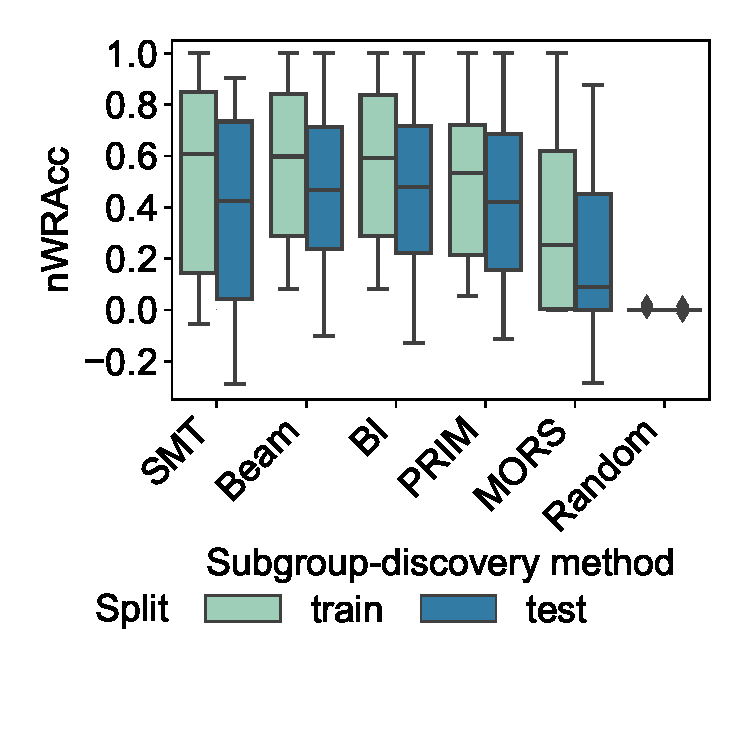
\includegraphics[width=\textwidth, trim=15 55 15 15, clip]{plots/csd-unconstrained-nwracc-all-datasets.pdf}
		\caption{All 27 datasets.}
		\label{fig:csd:unconstrained-nwracc-all-datasets}
	\end{subfigure}
	\hfill
	\begin{subfigure}[t]{0.48\textwidth}
		\centering
		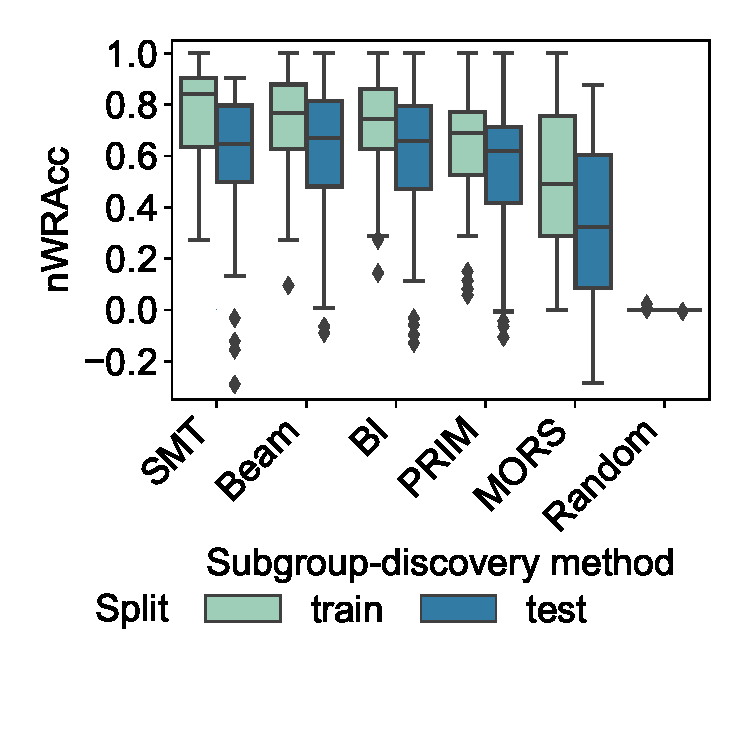
\includegraphics[width=\textwidth, trim=15 55 15 15, clip]{plots/csd-unconstrained-nwracc-no-timeout-datasets.pdf}
		\caption{17 datasets without \emph{SMT} timeouts.}
		\label{fig:csd:unconstrained-nwracc-no-timeout-datasets}
	\end{subfigure}
	\caption{
		Distribution of subgroup quality over datasets and cross-validation folds, by subgroup-discovery method.
		Results from the unconstrained experimental scenario.
	}
	\label{fig:csd:unconstrained-nwracc}
\end{figure}

\paragraph{Subgroup quality}

Figure~\ref{fig:csd:unconstrained-nwracc-all-datasets} compares subgroup quality for the six subgroup-discovery methods.
On the training set, the two heuristic search methods \emph{Beam} and \emph{BI} have roughly the same median nWRAcc as the solver-based search method \emph{SMT}.
In particular, the heuristics are even better than \emph{SMT} on some datasets but worse on others.
The former can happen when \emph{SMT} yields suboptimal solutions due to timeouts, as we analyze later (cf.~Section~\ref{sec:csd:evaluation:timeouts}).
However, even if we limit our analysis to the 17 datasets without \emph{SMT} timeouts, \emph{Beam} and \emph{BI} are still remarkably close to the optimum quality (cf.~Figure~\ref{fig:csd:unconstrained-nwracc-no-timeout-datasets}).
This result is not specific to \emph{SMT} but also affects any other exhaustive search method.
On the test set, \emph{Beam} and \emph{BI} are even better than \emph{SMT} on median, also excluding timeout datasets, since their training-test nWRAcc difference is smaller.
This result indicates that \emph{Beam} and \emph{BI} are less susceptible to overfitting, so their solutions generalize better.
In detail, the average difference between training-set nWRAcc and test-set nWRAcc is 0.122 for \emph{SMT}, 0.101 for \emph{BI}, 0.095 for \emph{Beam}, 0.094 for \emph{MORS}, 0.068 for \emph{PRIM}, and 0.001 for \emph{Random}.

The heuristic search method \emph{PRIM} yields worse subgroup quality than \emph{Beam} and \emph{BI}.
Although it follows an iterative subgroup-refinement procedure like the latter two methods, its refinement options are more limited.
In particular, \emph{PRIM} always has to remove a fixed fraction~$\alpha$ of data objects from the subgroup (cf.~Algorithm~\ref{al:csd:prim}), while \emph{Beam} and \emph{BI} can remove more or less.
Finally, all three heuristic search methods clearly beat the two baselines \emph{MORS} and \emph{Random}.
While \emph{Random} mostly yields the same quality as not restricting the subgroup at all, i.e., an nWRAcc of~0, \emph{MORS} is considerably above~0 and thus a suitable baseline for future studies comparing subgroup-discovery methods.

\begin{table}[t]
	\centering
	\caption{
		Aggregated runtime over datasets and cross-validation folds, by subgroup-discovery method.
		Results from the unconstrained experimental scenario.
	}
	\begin{subtable}{\textwidth}
		\centering
		\caption{
			All 27 datasets.
		}
		\begin{tabular}{lrrrrrr}
			\toprule
			Aggregate & BI & Beam & MORS & PRIM & Random & SMT \\
			\midrule
			Mean & 34.95~s & 30.47~s & 0.01~s & 1.26~s & 0.91~s & 849.02~s \\
			Standard deviation & 103.61~s & 85.69~s & 0.00~s & 1.51~s & 0.95~s & 929.60~s \\
			Median & 2.60~s & 2.95~s & 0.01~s & 0.66~s & 0.51~s & 254.21~s \\
			\bottomrule
		\end{tabular}
		\label{tab:csd:unconstrained-runtime-all-datasets}
	\end{subtable}
	\\ \vspace{\baselineskip}
	\begin{subtable}{\textwidth}
		\centering
		\caption{
			17 datasets without \emph{SMT} timeouts.
		}
		\begin{tabular}{lrrrrrr}
			\toprule
			Aggregate & BI & Beam & MORS & PRIM & Random & SMT \\
			\midrule
			Mean & 12.40~s & 11.77~s & 0.01~s & 1.29~s & 0.82~s & 168.13~s \\
			Standard deviation & 21.17~s & 20.47~s & 0.00~s & 1.62~s & 0.89~s & 243.11~s \\
			Median & 2.60~s & 2.95~s & 0.01~s & 0.80~s & 0.56~s & 57.23~s \\
			\bottomrule
		\end{tabular}
		\label{tab:csd:unconstrained-runtime-no-timeout-datasets}
	\end{subtable}
	\label{tab:csd:unconstrained-runtime}
\end{table}

\paragraph{Runtime}

Table~\ref{tab:csd:unconstrained-runtime} summarizes the runtimes of the subgroup-discovery methods.
On average, \emph{SMT} is an order of magnitude slower than \emph{Beam} and \emph{BI}, which are an order of magnitude slower than \emph{PRIM} and the baseline \emph{Random}.
The baseline \emph{MORS} runs in negligible time and thus is a good tool for instantaneously obtaining a lower bound on subgroup quality.
Taking subgroup quality into consideration, the heuristic search methods offer a good quality in a short time.
Among the three heuristics, \emph{PRIM} is the fastest but yields the lowest subgroup quality, so users should decide which runtime is acceptable.

For \emph{SMT}, the runtime not only comprises optimization but also formulating the optimization problem.
Since the latter depends on the dataset size, e.g., involves $O(m)$ constraints with length $O(n)$ each to define the subgroup-membership variables~$b_i$ (cf.~Equation~\ref{eq:csd:smt-constraint-subgroup-membership}), the preparation time can become considerable for large datasets.
In our experiments, formulating the \emph{SMT} problem took 45~s on average, with a maximum of 379~s.
This average preparation time is already greater than the average total runtime of the heuristics.

\begin{table}[t]
	\centering
	\caption{
		Spearman correlation between runtime and metrics for dataset size,
		over datasets and cross-validation folds, by subgroup-discovery method.
		Results from the unconstrained experimental scenario, using the 17 datasets without \emph{SMT} timeouts.
	}
	\begin{tabular}{lrrrr}
		\toprule
		Method & $\Sigma n^u$ & $m \cdot n$ & $m$ & $n$ \\
		\midrule
		BI & 0.95 & 0.51 & 0.32 & 0.67 \\
		Beam & 0.96 & 0.49 & 0.30 & 0.66 \\
		MORS & 0.27 & 0.57 & 0.51 & 0.26 \\
		PRIM & 0.84 & 0.56 & 0.29 & 0.76 \\
		Random & 0.58 & 0.69 & 0.42 & 0.77 \\
		SMT & 0.39 & 0.73 & 0.70 & 0.23 \\
		\bottomrule
	\end{tabular}
	\label{tab:csd:unconstrained-runtime-correlation}
\end{table}

To determine which factors influence runtime, we analyze the Spearman correlation between runtime and four simple metrics for dataset size.
In particular, Table~\ref{tab:csd:unconstrained-runtime-correlation} considers the number of data objects~$m$, the number of features~$n$, the product of these two quantities~$m \cdot n$, and the number of unique values per feature summed over the features~$\Sigma n^u$.
For the three heuristic search methods, the latter metric shows a high correlation to runtime, while \emph{SMT} exhibits the highest runtime correlation to~$m \cdot n$.

\subsection{Solver Timeouts}
\label{sec:csd:evaluation:timeouts}

In this section, we evaluate the impact of solver timeouts for \emph{SMT} search.

\begin{figure}[t]
	\centering
	\begin{subfigure}[t]{0.48\textwidth}
		\centering
		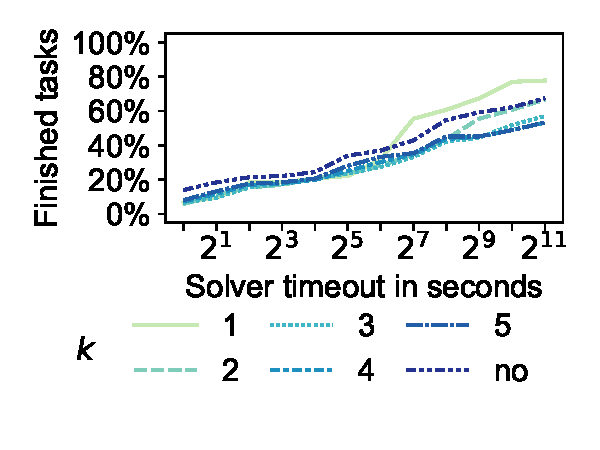
\includegraphics[width=\textwidth, trim=15 25 15 10, clip]{plots/csd-timeouts-finished-tasks.pdf}
		\caption{
			Frequency of finished \emph{SMT} tasks over datasets and cross-validation folds, by feature cardinality~$k$.
		}
		\label{fig:csd:timeouts-finished-tasks}
	\end{subfigure}
	\hfill
	\begin{subfigure}[t]{0.48\textwidth}
		\centering
		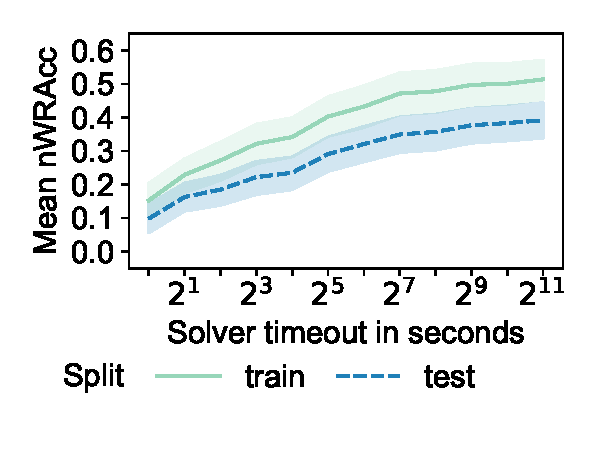
\includegraphics[width=\textwidth, trim=15 25 15 10, clip]{plots/csd-timeouts-nwracc.pdf}
		\caption{
			Mean subgroup quality, with 95\% confidence intervals based on datasets and cross-validation folds.
			Results from the unconstrained experimental scenario.
		}
		\label{fig:csd:timeouts-nwracc}
	\end{subfigure}
	\caption{
		Impact of solver timeouts for \emph{SMT} as the subgroup-discovery method.
		Results from the search for original subgroups.
	}
	\label{fig:csd:timeouts}
\end{figure}

\paragraph{Finished tasks}

Figure~\ref{fig:csd:timeouts-finished-tasks} displays how many of the \emph{SMT} optimization tasks for original subgroups finished within the evaluated solver timeouts.
Besides the unconstrained tasks, we also consider different feature-cardinality thresholds, though the overall trend is the same.
In particular, the number of finished tasks only increases slowly over time, and some tasks take orders of magnitude longer than others.
E.g., in the unconstrained experimental scenario, 21.5\% of the \emph{SMT} tasks finished within 4~s, 24.4\% within 16~s, 37.0\% within 64~s, 54.8\% within 256~s, and 62.2\% within 1024~s.
For the maximum setting of 2048~s, 67.4\% of the \emph{SMT} tasks finished, and 17 out of 27 datasets did not encounter timeouts (cf.~Table~\ref{tab:csd:datasets}).

\paragraph{Subgroup quality}

Figure~\ref{fig:csd:timeouts-nwracc} visualizes the subgroup quality over solver timeouts for unconstrained \emph{SMT} search.
This plot uses the quality of the optimal solution for finished tasks and of the currently best solution for unfinished tasks.
As for the number of finished tasks (cf.~Figure~\ref{fig:csd:timeouts-finished-tasks}), the largest gains occur in the first minute.
E.g., the mean test-set nWRAcc over datasets and cross-validation folds is 0.10 for 1~s, 0.19 for 4~s, 0.24 for 16~s, 0.32 for 64~s, and 0.39 for the maximum solver timeout of 2024~s.
The main cause for this trend is that many tasks finish relatively early (cf.~Figure~\ref{fig:csd:timeouts-finished-tasks}), and finished tasks cannot improve their quality for higher solver timeouts.
In contrast, if we only consider the tasks where the solver did not finish even within the maximum solver timeout, the quality increase of the currently best solution over time is marginal.

Further, even \emph{SMT} with a timeout does not compare favorably to fast heuristic search methods.
E.g., with a solver timeout of 64~s, corresponding to an average overall runtime of 88~s, \emph{SMT} achieves a mean training-set nWRAcc of 0.43, compared to 0.56 for \emph{Beam} with an average runtime of 30~s (cf.~Table~\ref{tab:csd:unconstrained-runtime-all-datasets}).
Finally, setting a lower solver timeout decreases overfitting, i.e., the difference between training-set nWRAcc and test-set nWRAcc increases over time (cf.~Figure~\ref{fig:csd:timeouts-nwracc}).
However, since the test-set nWRAcc still increases with the timeout, choosing lower timeouts does not help quality-wise.

\subsection{Feature-Cardinality Constraints}
\label{sec:csd:evaluation:cardinality}

In this section, we compare all subgroup-discovery methods in the experimental scenario with feature-cardinality constraints.
\emph{SMT} uses its default solver timeout of 2048~s.

\begin{figure}[t]
	\centering
	\begin{subfigure}[t]{0.48\textwidth}
		\centering
		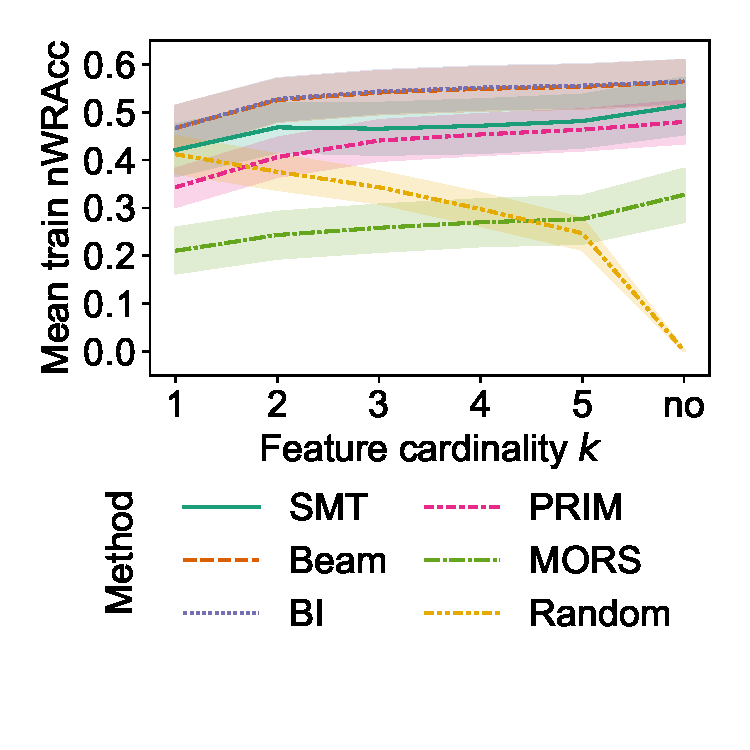
\includegraphics[width=\textwidth, trim=15 55 15 15, clip]{plots/csd-cardinality-train-nwracc-all-datasets.pdf}
		\caption{All 27 datasets, training set.}
		\label{fig:csd:cardinality-train-nwracc-all-datasets}
	\end{subfigure}
	\hfill
	\begin{subfigure}[t]{0.48\textwidth}
		\centering
		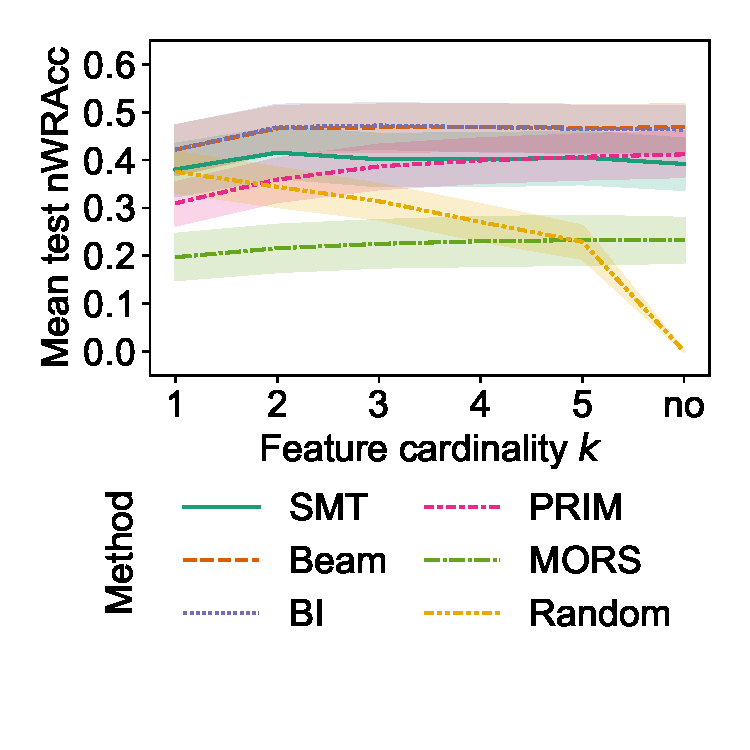
\includegraphics[width=\textwidth, trim=15 55 15 15, clip]{plots/csd-cardinality-test-nwracc-all-datasets.pdf}
		\caption{All 27 datasets, test set.}
		\label{fig:csd:cardinality-test-nwracc-all-datasets}
	\end{subfigure}
	\\
	\begin{subfigure}[t]{0.48\textwidth}
		\centering
		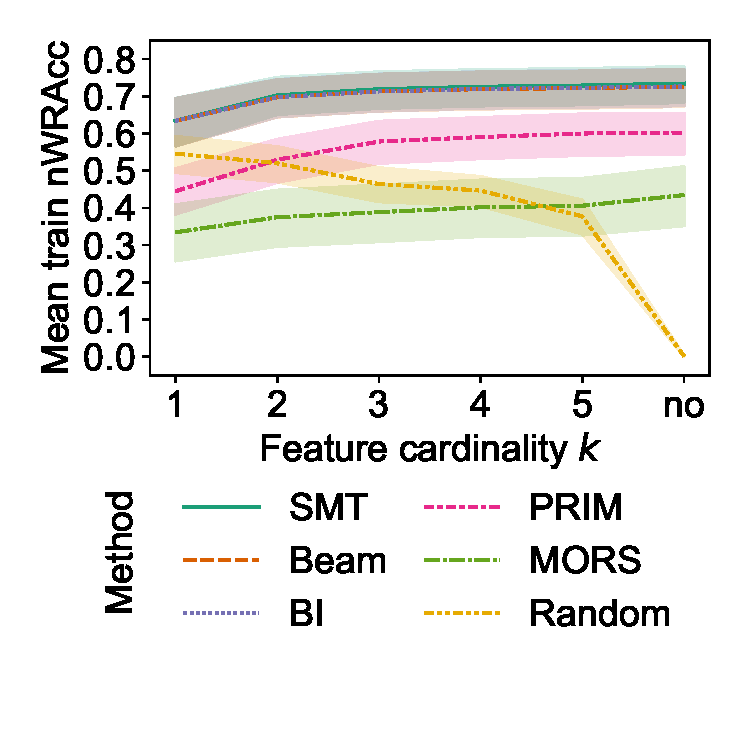
\includegraphics[width=\textwidth, trim=15 55 15 15, clip]{plots/csd-cardinality-train-nwracc-no-timeout-datasets.pdf}
		\caption{13 datasets without \emph{SMT} timeouts, training set.}
		\label{fig:csd:cardinality-train-nwracc-no-timeout-datasets}
	\end{subfigure}
	\hfill
	\begin{subfigure}[t]{0.48\textwidth}
		\centering
		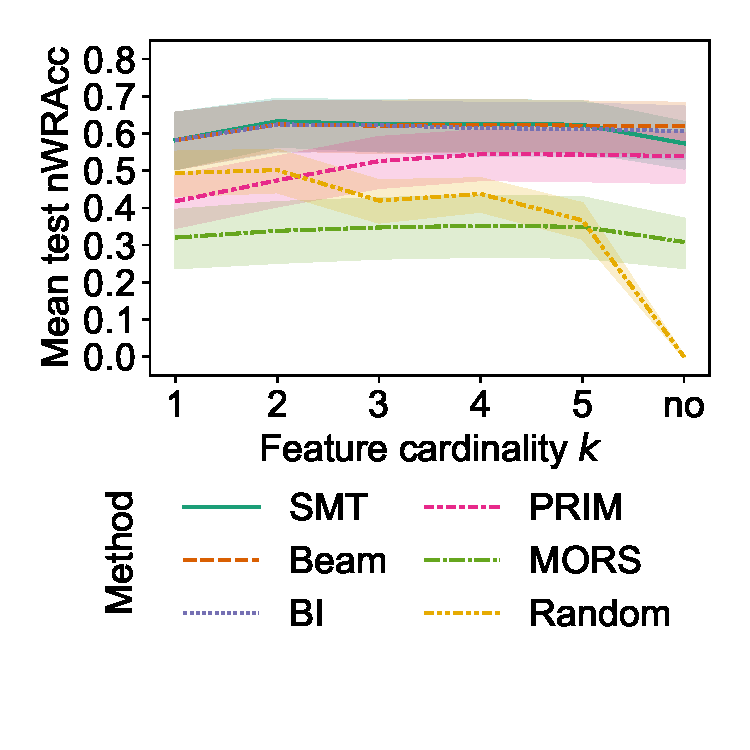
\includegraphics[width=\textwidth, trim=15 55 15 15, clip]{plots/csd-cardinality-test-nwracc-no-timeout-datasets.pdf}
		\caption{13 datasets without \emph{SMT} timeouts, test set.}
		\label{fig:csd:cardinality-test-nwracc-no-timeout-datasets}
	\end{subfigure}
	\caption{
		Mean subgroup quality, with 95\% confidence intervals based on datasets and cross-validation folds, by subgroup-discovery method and feature cardinality~$k$.
		Results from the search for original subgroups.
	}
	\label{fig:csd:cardinality-nwracc}
\end{figure}

\paragraph{Subgroup quality}

Figure~\ref{fig:csd:cardinality-nwracc} displays the mean subgroup quality, averaging over datasets and cross-validation folds, for different values of the feature-cardinality threshold~$k$.
For most subgroup-discovery methods, mean training-set nWRAcc (cf.~Figure~\ref{fig:csd:cardinality-train-nwracc-all-datasets}) increases with~$k$, though the marginal utility decreases.
In particular, even with $k=1$, the mean nWRAcc is already clearly above 50\% of the nWRAcc achieved with all features.
Further, the quality increase between $k=1$ and $k=2$ is usually the largest.
On the test set (cf.~Figure~\ref{fig:csd:cardinality-test-nwracc-all-datasets}), the benefit of setting a larger~$k$ is even smaller.
E.g., the mean test-set nWRAcc of \emph{Beam}, \emph{BI}, and \emph{SMT} barely improves beyond $k=2$.
These results indicate that sparse subgroup descriptions already yield a high subgroup quality.
The baseline \emph{Random} even improves subgroup quality with lower~$k$ due to its design (cf.~Algorithm~\ref{al:csd:random-search}):
\emph{Random} samples bounds independently for each feature.
The more features are used in the subgroup description, the smaller the expected number of data objects in the subgroup becomes.
However, the number of subgroup members is one factor in WRAcc (cf.~Equation~\ref{eq:csd:wracc}).

Figures~\ref{fig:csd:cardinality-train-nwracc-all-datasets} and~\ref{fig:csd:cardinality-test-nwracc-all-datasets} also reveal that the heuristic search methods \emph{Beam} and \emph{BI} still yield higher average subgroup quality than the solver-based search \emph{SMT} due to timeouts, for any feature-cardinality setting.
Even excluding the datasets with \emph{SMT} timeouts (cf.~Figures~\ref{fig:csd:cardinality-train-nwracc-no-timeout-datasets} and~\ref{fig:csd:cardinality-test-nwracc-no-timeout-datasets}), these two heuristics yield nearly the same average subgroup quality as \emph{SMT} for constrained~$k$ and have an advantage on the test set with unconstrained~$k$.
The heuristic \emph{PRIM} exhibits a larger increase of subgroup quality over~$k$ than \emph{Beam} and \emph{BI}, thereby narrowing the quality gap to the latter.
The baseline \emph{MORS} displays the least effect of~$k$ on mean test-set nWRAcc, showing very stable subgroup quality.

Finally, the results indicate that limiting~$k$ reduces overfitting.
For example, \emph{Beam} has a mean training-test nWRAcc difference of 0.095 without limiting~$k$, 0.073 for $k=3$, and 0.045 for $k=1$.
The increasing tendency to overfit with larger~$k$ explains why mean training-set nWRAcc increases more than mean test-set nWRAcc over~$k$ in Figure~\ref{fig:csd:cardinality-nwracc}.
\emph{PRIM} shows the smallest increase of overfitting over~$k$, \emph{MORS} and \emph{SMT} the largest.

\begin{table}[t]
	\centering
	\caption{
		Mean runtime over datasets and cross-validation folds, by subgroup-discovery method and feature cardinality~$k$.
		Results from the search for original subgroups.
	}
	\begin{tabular}{lrrrrrr}
		\toprule
		$k$ & BI & Beam & MORS & PRIM & Random & SMT \\
		\midrule
		1 & 7.81~s & 6.81~s & 0.01~s & 0.08~s & 0.63~s & 648.16~s \\
		2 & 11.74~s & 10.06~s & 0.01~s & 0.17~s & 0.64~s & 911.28~s \\
		3 & 14.20~s & 12.78~s & 0.01~s & 0.26~s & 0.65~s & 1091.75~s \\
		4 & 16.68~s & 14.65~s & 0.01~s & 0.35~s & 0.66~s & 1113.40~s \\
		5 & 18.66~s & 16.12~s & 0.01~s & 0.46~s & 0.66~s & 1117.39~s \\
		no & 34.95~s & 30.47~s & 0.01~s & 1.26~s & 0.91~s & 849.02~s \\
		\bottomrule
	\end{tabular}
	\label{tab:csd:cardinality-runtime}
\end{table}

\paragraph{Runtime}

As Table~\ref{tab:csd:cardinality-runtime} displays, the heuristic search methods \emph{Beam}, \emph{BI}, and \emph{PRIM} become faster the smaller~$k$ is.
The baseline \emph{Random} shows a similar trend, though less prominent, while \emph{MORS} yields results instantaneously in any case.
In contrast, the picture for the solver-based search method \emph{SMT} is less clear.
While its average runtime clearly increases from $k=1$ till $k=3$, it roughly remains constant for $k \in \{4, 5\}$ and even decreases without a feature-cardinality constraint, only remaining higher than for $k = 1$.

\subsection{Alternative Subgroup Descriptions}
\label{sec:csd:evaluation:alternatives}

In this section, we analyze alternative subgroup descriptions for \emph{Beam} and \emph{SMT}.
Both employ a feature cardinality of~$k=3$.
\emph{SMT} uses its default solver timeout of 2048~s.

\begin{figure}[t]
	\centering
	\begin{subfigure}[t]{0.48\textwidth}
		\centering
		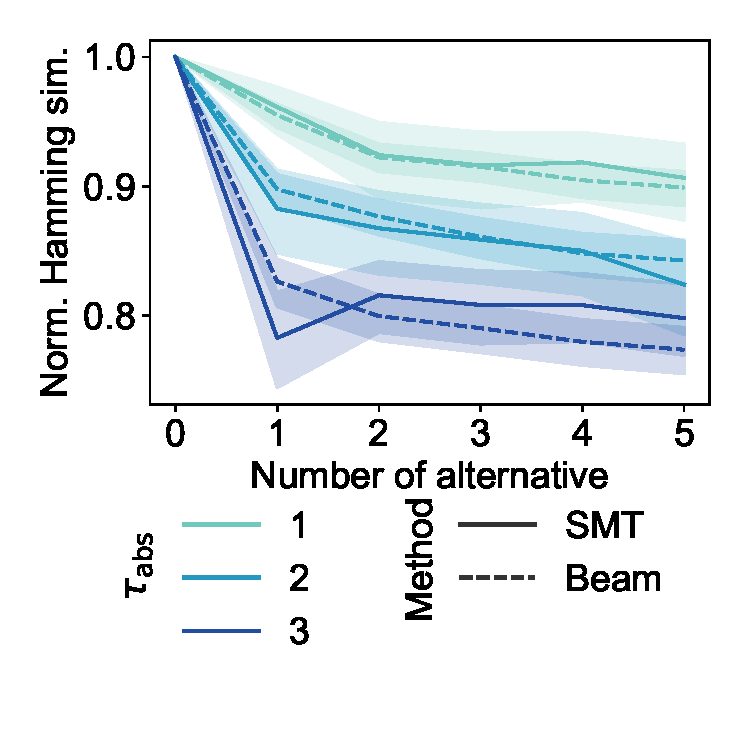
\includegraphics[width=\textwidth, trim=15 50 15 15, clip]{plots/csd-alternatives-hamming.pdf}
		\caption{Normalized Hamming similarity.}
		\label{fig:csd:alternatives-hamming}
	\end{subfigure}
	\hfill
	\begin{subfigure}[t]{0.48\textwidth}
		\centering
		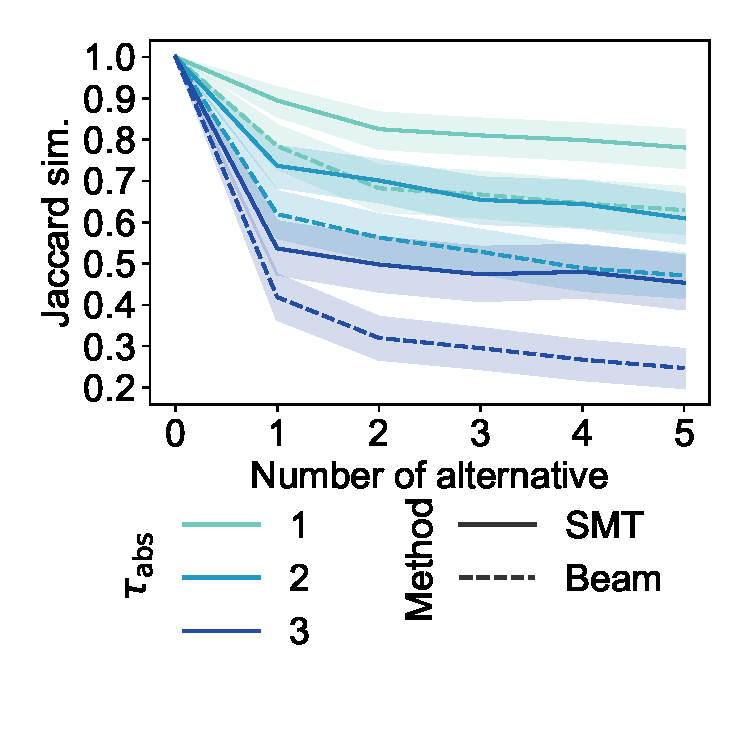
\includegraphics[width=\textwidth, trim=15 50 15 15, clip]{plots/csd-alternatives-jaccard.pdf}
		\caption{Jaccard similarity.}
		\label{fig:csd:alternatives-jaccard}
	\end{subfigure}
	\caption{
		Mean subgroup similarity of alternative subgroup descriptions to the original subgroup, with 95\% confidence intervals based on datasets and cross-validation folds, by subgroup-discovery method, number of alternative, and dissimilarity threshold~$\tau_{\text{abs}}$.
	}
	\label{fig:csd:alternatives-similarity}
\end{figure}

\paragraph{Subgroup similarity}

Figure~\ref{fig:csd:alternatives-similarity} visualizes the average similarity between the original subgroups and those induced by alternative subgroup descriptions.
As expected, the subgroup-membership similarity decreases the more alternatives one desires and the more the selected features in subgroup descriptions should differ.
Further, the decrease is strongest from the original subgroup, i.e., the zeroth alternative, to the first alternative but smaller beyond.
This observation indicates that one may find several alternative subgroup descriptions of comparable similarity to the original.

These trends hold for both similarity measures, i.e., the normalized Hamming similarity we optimize (cf.~Equation~\ref{eq:csd:hamming-general} and Figure~\ref{fig:csd:alternatives-hamming}) as well as the Jaccard similarity (cf.~Equation~\ref{eq:csd:jaccard} and Figure~\ref{fig:csd:alternatives-jaccard}).
The latter yields lower similarity values than the former since it ignores data objects that are not contained in either of the two compared subgroups.
Further, the observed trends exist for the solver-based search method \emph{SMT} as well as the heuristic search method \emph{Beam}.
\emph{SMT} yields clearly more similar subgroups than \emph{Beam} for the Jaccard similarity, while the normalized Hamming similarity does not show a clear winner.

\begin{figure}[t]
	\centering
	\begin{subfigure}[t]{0.48\textwidth}
		\centering
		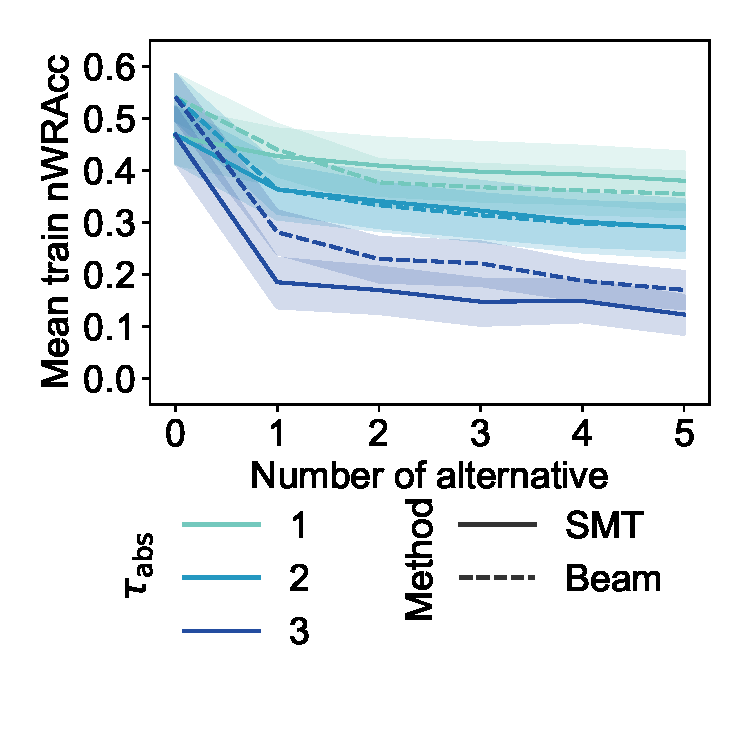
\includegraphics[width=\textwidth, trim=15 50 15 15, clip]{plots/csd-alternatives-train-nwracc.pdf}
		\caption{Training set.}
		\label{fig:csd:alternatives-train-nwracc}
	\end{subfigure}
	\hfill
	\begin{subfigure}[t]{0.48\textwidth}
		\centering
		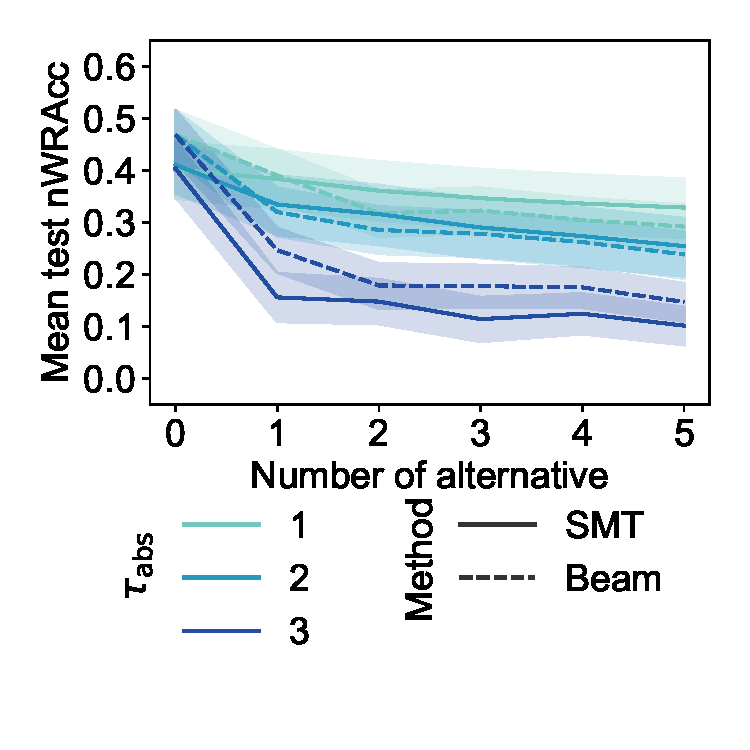
\includegraphics[width=\textwidth, trim=15 50 15 15, clip]{plots/csd-alternatives-test-nwracc.pdf}
		\caption{Test set.}
		\label{fig:csd:alternatives-test-nwracc}
	\end{subfigure}
	\caption{
		Mean subgroup quality of alternative subgroup descriptions, with 95\% confidence intervals based on datasets and cross-validation folds, by subgroup-discovery method, number of alternative, and dissimilarity threshold~$\tau_{\text{abs}}$.
	}
	\label{fig:csd:alternatives-nwracc}
\end{figure}

\paragraph{Subgroup quality}

The average subgroup quality of alternative subgroup descriptions (cf.~Figure~\ref{fig:csd:alternatives-nwracc}) shows similar trends as subgroup similarity (cf.~Figure~\ref{fig:csd:alternatives-similarity}) and the quality of alternative feature sets in our previous chapter (cf.~Figure~\ref{fig:afs:impact-num-alternatives-tau-quality}).
In particular, quality decreases over the dissimilarity threshold~$\tau_{\text{abs}}$ and over the number of alternatives~$a$, with the largest decrease to the first alternative.
For the highest dissimilarity threshold~$\tau_{\text{abs}} = 3$, \emph{Beam} consistently yields higher average quality than \emph{SMT} for the original subgroup and each alternative.
In contrast, the other two values of the dissimilarity threshold do not clearly favor either method.
The observed trends on the test set (cf.~Figure~\ref{fig:csd:alternatives-test-nwracc}) are very similar to those on the training set (cf.~Figure~\ref{fig:csd:alternatives-train-nwracc}).
For both subgroup-discovery methods, overfitting, as measured by the training-test difference in nWRAcc, is lower for the alternative subgroup descriptions than for the original subgroups.
This phenomenon may result from the alternatives not directly optimizing subgroup quality.

\begin{table}[t]
	\centering
	\caption{
		Mean runtime over datasets and cross-validation folds, by subgroup-discovery method, dissimilarity threshold~$\tau_{\text{abs}}$, and number of alternative.
		Results from the search for alternative subgroup descriptions.
	}
	\begin{tabular}{llrrrrrr}
		\toprule
		\multirow{2}{*}{Method} & \multirow{2}{*}{$\tau_{\text{abs}}$} & \multicolumn{6}{c}{Number of alternative} \\
		\cmidrule(lr){3-8}
		& &  0 & 1 & 2 & 3 & 4 & 5 \\
		\midrule
		\multirow[t]{3}{*}{Beam} & 1 & 12.8~s & 8.0~s & 7.6~s & 7.3~s & 7.3~s & 7.3~s \\
		& 2 & 12.8~s & 7.7~s & 7.4~s & 7.2~s & 7.0~s & 6.8~s \\
		& 3 & 12.8~s & 5.8~s & 5.1~s & 4.7~s & 4.1~s & 3.5~s \\
		\multirow[t]{3}{*}{SMT} & 1 & 1091.7~s & 166.0~s & 221.5~s & 239.6~s & 258.1~s & 277.9~s \\
		& 2 & 1105.2~s & 377.5~s & 463.5~s & 537.5~s & 599.4~s & 658.3~s \\
		& 3 & 1107.4~s & 869.1~s & 670.8~s & 597.6~s & 588.1~s & 557.6~s \\
		\bottomrule
	\end{tabular}
	\label{tab:csd:alteratives-runtime}
\end{table}

\paragraph{Runtime}

Table~\ref{tab:csd:alteratives-runtime} displays the average runtime for searching original subgroups and alternative subgroup descriptions.
The search for alternatives is faster for both analyzed search methods, i.e., \emph{Beam} and \emph{SMT}.
As for the original subgroups, \emph{Beam} search for alternatives is one to two orders of magnitude faster than the solver-based \emph{SMT} search.
For \emph{Beam}, runtime tends to decrease over the number of alternatives, while \emph{SMT} shows a less clear behavior.
In particular, its runtime increases over alternatives for~$\tau_{\text{abs}} \in \{1, 2\}$, i.e., settings that allow reusing features from previous subgroup descriptions.
In contrast, runtime decreases over alternatives for $\tau_{\text{abs}} = k = 3$, which forbids reusing any feature selected before.
Finally, the number of \emph{SMT} tasks finished within the solver timeout shows trends corresponding to the runtime.
In particular, there are more finished tasks when searching for alternative subgroup descriptions than for original subgroups.

\subsection{Summary}
\label{sec:csd:evaluation:summary}

\paragraph{Unconstrained subgroup discovery (cf.~Section~\ref{sec:csd:evaluation:unconstrained})}

We recommend using heuristic search methods rather than solver-based search.
In particular, \emph{Beam} and \emph{BI} were an order of magnitude faster than \emph{SMT} and still yielded higher test-set subgroup quality since they overfit less.
The latter result not only impedes \emph{SMT} but other exhaustive search methods as well.
\emph{PRIM} was faster than \emph{Beam} and \emph{BI} but yielded lower subgroup quality.
Our novel baseline \emph{MORS} provided instantaneous, non-trivial lower bounds for subgroup quality.

\paragraph{Solver timeouts (cf.~Section~\ref{sec:csd:evaluation:timeouts})}

Setting larger solver timeouts showed a decreasing marginal utility regarding the number of finished \emph{SMT} tasks and subgroup quality, i.e., most gains occurred within the first dozens of seconds.
About half the \emph{SMT} tasks that finished at all finished in under a minute.
However, the average subgroup quality with this solver timeout was lower than for heuristic search methods with even lower runtime.

\paragraph{Feature-cardinality constraints (cf.~Section~\ref{sec:csd:evaluation:cardinality})}

Using more features in subgroup descriptions showed a decreasing marginal utility regarding subgroup quality.
For \emph{Beam}, \emph{BI}, and \emph{SMT}, test-set subgroup quality was already close to the unconstrained scenario at $k=2$, while \emph{PRIM} benefited more from larger~$k$.
A smaller~$k$ made the heuristic search methods faster and generally reduced overfitting.
\emph{MORS} showed stable test-set subgroup quality regarding~$k$, while \emph{Random} even increased subgroup quality with smaller~$k$.

\paragraph{Alternative subgroup descriptions (cf.~Section~\ref{sec:csd:evaluation:alternatives})}

The heuristic \emph{Beam} was one to two orders of magnitude faster than solver-based \emph{SMT} when searching for alternative subgroup descriptions, while both search methods found alternatives faster than original subgroups.
The quality and similarity of alternatives strongly depended on the number of alternatives~$a$ and the dissimilarity threshold~$\tau_{\text{abs}}$.
The difference in quality and similarity between the original and the first alternative was higher than among the first few alternatives.
